\chapter{Format of the Input Files}

\section{Introduction}

In order to run a simulation you need several input-files:
\begin{itemize}
\item{\verb=`simulation.input'=}\\
This file contains the information on the type of simulation, the amount of steps, the framework name, number of unit cells
in each directions, the used molecules, the type of used Monte-Carlo moves etc.\
\item{\verb=`structure-name.cif'=}\\
If a framework (e.g.\ a zeolite or MOF) is used, then the definition of the structure needs to be provided. CIF-files are supported and the default input.
The name of the file should be equal to the one provided in \verb=`simulation.input'=, e.g.\ IRMOF-1.cif if \verb=`Frameworkname IRMOF-1'= is listed in
\verb=`simulation.input'=.
\item{\verb=`pseudo_atoms.def'=}\\
The \verb=`pseudo_atoms.def'= file list all the information on used pseudo-atoms, e.g.\ charge, mass. Usually a pseudo-atom is an atom, but there are exceptions
like united atoms (where CH3 is lumped into one unit) and off-atom sites in Tip5p water that represent oxygen lone pairs.
Because in CIF-files for frameworks you can provide also
information on atoms, there is no need to list framework atoms here if a CIF-file is used. On reading the CIF-file these defined atoms are added to the
pseudo-atoms. If also provided in the \verb=`pseudo_atoms.def'= then the definition in the \verb=`pseudo_atoms.def'= file has priority.
\item{\verb=`force_field_mxing_rules.def'=,\verb=`force_field.def'=}\\
The force field defined on the pseudo-atoms in \verb=`pseudo_atoms.def'=. These files list the Van der Waals potential types, the parameters, whether to
use tail-corrections, whether to shift to zero at the cutoff, and the type of mixing rule.
Force fields in literature are usually published in two forms: 1) a list of potentials parameters per atom and a mixing rule, or 2) pairs of atoms and parameters.
The first option corresponds to the file \verb=`force_field_mxing_rules.def'= and the latter option to the file \verb=`force_field.def'=. You can use both
at the same time, where \verb=`force_field.def'= has precedence over \verb=`force_field_mxing_rules.def'=.
\item{\verb=`molecule-name.def'=}\\
The definition of the used molecules.
The name of the file should be equal to the one provided in \verb=`simulation.input'=, e.g.\ propane.def if \verb=`MoleculeName propane'= is listed in
\verb=`simulation.input'=.
\item{\verb=zframework.def'=}\\
Used for a flexible framework to define all the bonds, bends, torsions, core-shells, etc.
\end{itemize}

The format of these files will be described in the remaining sections. Chapter \ref{Examples: chapter} provides lots of examples to see everything in action.
In addition to the input-files you will need either a \verb=`run'= file that is executable, or a queuing-script to submit the job to the queue
(see \ref{Introduction: running RASPA}).

\section{Simulation input}

Leading spaces and comments at the end of each line are omitted. Empty lines are skipped, 
and case is not important except in file names (i.e. framework and molecule names).

\subsection*{Simulation types}
\begin{itemize}
\item{SimulationType MonteCarlo}\\
Starts the Monte Carlo part of RASPA. The particular ensemble is not specified but implicitly deduced from
the specified Monte Carlo moves. Note that a MD-move can be used for hybrid MC/MD.
\item{SimulationType MolecularDynamics}\\
Starts the Molecular Dynamics part of RASPA. The ensemble is explicitly specified.
\item{SimulationType Spectra}\\
Starts the computation of the vibrational analysis. Possible options include infra red spectrum at zero Kelvin,
powder diffraction, and mode analysis.
\item{SimulationType Minimization}\\
Starts the minimization routine. It produces configurations and crystal structures at zero Kelvin.
\item{SimulationType Visualization}\\
Output VTK-files for snapshots and crystal structures, including energy surface pictures.
\item{SimulationType BarrierCrossing}\\
Routine for the dynamical correction of dynamically corrected Transition State Theory.
\item{SimulationType Numerical}\\
Computes all the forces numerically from the energy and compares them to the analytical expressions.
Also the strain-derivative tensor (related to the stress tensor), and the second derivative of
the energy with respect to strain, as well as the Hessian matrix can be checked.
\item{SimulationType MakeGrid}\\
Creates pre-tabulated energy-grids for use in rigid frameworks.
\end{itemize}

\subsection*{Simulation duration}
\begin{itemize}
\item{NumberOfCycles [int]}\\
The number of cycles for the production run. 
For Monte Carlo a cycle consists of $N$ steps, where $N$ is the amount of
molecules with a minimum of 20 steps. This means that on average during each cycle on each molecule a
Monte Carlo move has been attempted (either successful or unsuccessful). For MD the number of cycles
is simply the amount of integration steps.
\item{NumberOfInitializationCycles [int]}\\
The number of cycles used to initialize the system using Monte Carlo. This can be used for both Monte Carlo
as well as Molecular Dynamics to quickly equilibrate the positions of the atoms in the system.
\item{NumberOfEquilibrationCycles [int]}\\
For Molecular Dynamics  it is the number of MD steps to equilibrate the velocities in the systems. After this 
equilibration the production run is started. For Monte Carlo, in particular CFMC, the equilibration-phase is used
to measure the biasing factors.
\end{itemize}

\subsection*{Restart and crash-recovery}
\begin{itemize}
\item{RestartFile [yes$|$no]}\\
Reads the positions, velocities, and force from the directory `RestartInitial'. Any creation of molecules
in the `simulation.input' file will be in addition and after this first read from file. This is useful to
load initial positions of cations for example, and after that create adsorbates. The restart file
is written at `PrintEvery' intervals.
\item{ContinueAfterCrash [yes$|$no]}\\
Write a binary file containing the complete status of the program. 
The file name is `binary\_restart.dat' and is located in the directory `CrashRestart'.
With this option to `yes' the presence of this file will result in continuation from
the point where the program was at the moment of outputting this file.
The file can be quite big (several hundreds of megabytes) and will be outputted every
`WriteBinaryRestartFileEvery' cycles.
\item{WriteBinaryRestartFileEvery [int]}\\
The output frequency (i.e. every [int] cycles) of the crash-recovery file.
\end{itemize}

\subsection*{Printing options}
\begin{itemize}
\item{PrintEvery [int]}\\
Prints the loadings (when a framework is present) and energies every [int] cycles. For MD information
like energy conservation and stress are printed.
\item{PrintPropertiesEvery [int]}\\
Output running averages of many properties (i.e. Henry coefficients and elastic constants).
\item{PrintForcefieldToOutput [yes$|$no]}\\
Prints the force field information to the output-file.
Default: yes.
\item{PrintPseudoAtomsToOutput [yes$|$no]}\\
Prints the pseudo-atom information to the output-file.
Default: yes.
\item{PrintMoleculeDefinitionToOutput [yes$|$no]}\\
Prints the molecule definition information to the output-file.
Default: yes.
\end{itemize}

\subsection*{Force field definitions}
\begin{itemize}
\item{ChargeFromChargeEquilibration [yes$|$no]}\\
Compute the charges of the framework using the `charge-equilibration'-method.
\item{SymmetrizeFrameworkCharges [yes$|$no]}\\
All charges of the framework are made equivalent for equivalent framework atoms. 
Using regular charge-equilibration the charges are different for symmtrically equivalent
framework atoms, and this options restores the symmetry.
\item{ForceField [string]}\\
Reads in the force field [string], first the file `pseudo\_atoms.def' is read, then 
`force\_field\_mixing\_rules.def' and finally `force\_field.def'. The latter overwrites
general settings for interactions based on mixing rules with specific ones for individual
interactions. 

Note that if any of these files are in the working directory then these will read and used instead of the
ones in `\$\{RASPA\_DIR\}/simulations/share/raspa/forcefield/[string]'.

\item{CutOffVDW [real]}\\
The cutoff of the Van der Waals potentials. Interactions longer then this distance are omitted from the
energy and force computations. The potential can either be shifted to zero at the cutoff, or interactions
can just neglected after the cut off, or the remainder of the potential energy can be approximated using
tail corrections. This is specified in the force field files and can be specified globally or
for each interaction individually.
\item{CutOffVDWSwitch [real]}\\
The distance at which VDW switching will start. The smoothing will make sure the value and derivatives are zero at the cutoff.
The default: 0.9 times the CutOff.
\item{CutOffChargeCharge [real]}\\
The cutoff of the charge-charge potential. The potential is truncated at the cutoff and only shifted when `ChargeMethod CoulombShifted'
or `ChargeMethod CoulombSmoothed' is used.
No tail-corrections are (or can be) applied. The only way to include the long-range part is to use `ChargeMethod Ewald'.
The parameter is also used in combination with the
Ewald precision to compute the number of wave vectors and Ewald parameter $\alpha$.
For the Ewald summation using rather large unit cells, a charge-charge cutoff of about half the smallest box-length would be advisable
in order to avoid the use of an excessive amount of wave-vectors in Fourier space. For non-Ewald methods the cutoff should be as large
as possible (greater than about 30 \AA).
\item{CutOffChargeChargeSwitch [real]}\\
The distance at which charge-charge switching will start. The smoothing will make sure the value and derivatives are zero at the cutoff.
The default: 0.65 times the CutOff.
\item{CutOffChargeBondDipole [real]}\\
The cutoff of the charge-bonddipole potential.
\item{CutOffChargeBondDipoleSwitch [real]}\\
The distance at which charge-bonddipole switching will start. The smoothing will make sure the value and derivatives are zero at the cutoff.
The default: 0.70 times the CutOff.
\item{CutOffBondDipoleBondDipole [real]}\\
The cutoff of the bonddipole-bonddipole potential.
\item{CutOffBondDipoleBondDipoleSwitch [real]}\\
The distance at which bonddipole-bonddipole switching will start. The smoothing will make sure the value and derivatives are zero at the cutoff.
The default: 0.75 times the CutOff.


\item{OmitAdsorbateAdsorbateVDWInteractions [yes$|$no]}\\
Omits the Van der Waals interactions between adsorbates.
\item{OmitAdsorbateAdsorbateCoulombInteractions [yes$|$no]}\\
Omits the Coulombic (i.e. Ewald) interactions between adsorbates.
\item{OmitInterMolecularInteractions [yes$|$no]}\\
Omits the interactions between all molecules (only interactions with the framework). This also
works with the Ewald summation on. The options implies the setting of both
\begin{itemize}
  \item{OmitAdsorbateAdsorbateVDWInteractions [yes$|$no]}
  \item{OmitAdsorbateAdsorbateCoulombInteractions [yes$|$no]}
\end{itemize}
\item{InternalFrameworkLennardJonesInteractions [yes$|$no]}\\
Compute the Van der Waals interaction of the flexible framework. The Demontis flexible model for silicalite
is defined with only bond, bend, and torsion for example. One can use this option and also use
`Charge None'.
\item{$\begin{array}{l}\text{RemoveBondNeighboursFromLongRangeInteraction [yes$|$no]}\\
      \text{RemoveBendNeighboursFromLongRangeInteraction [yes$|$no]}\\
      \text{RemoveTorsionNeighboursFromLongRangeInteraction [yes$|$no]}\end{array}$}\\
After construction of the connectivity table all interactions are removed from Van der Waals and charge
interactions that are defined as 1-2 (i.e. bonds), 1-3 (i.e. bends, Urey-Bradley) and 1-4 (i.e. torsion, inversion-bend) respectively.
\item{Remove12NeighboursFromChargeChargeInteraction [yes$|$no]\\
      Remove13NeighboursFromChargeChargeInteraction [yes$|$no]\\
      Remove14NeighboursFromChargeChargeInteraction [yes$|$no]}\\
Remove all 1-2, 1-3, and/or 1-4 interactions within the framework from the long-range charge-charge
interaction within the flexible framework respectively.
\item{Remove12NeighboursFromChargeBondDipoleInteraction [yes$|$no]\\
      Remove13NeighboursFromChargeBondDipoleInteraction [yes$|$no]\\
      Remove14NeighboursFromChargeBondDipoleInteraction [yes$|$no]}\\
Remove all 1-2, 1-3, and/or 1-4 interactions within the framework from the long-range charge-bond dipole
interaction within the flexible framework respectively.
\item{Remove12NeighboursFromBondDipoleBondDipoleInteraction [yes$|$no]\\
      Remove13NeighboursFromBondDipoleBondDipoleInteraction [yes$|$no]\\
      Remove14NeighboursFromBondDipoleBondDipoleInteraction [yes$|$no]}\\
Remove all 1-2, 1-3, and/or 1-4 interactions within the framework from the long-range bond dipole-bond dipole
interaction within the flexible framework respectively.
\end{itemize}

\subsection*{Thermostat and barostat parameters}
\begin{itemize}
\item{ExternalTemperature [list-of-reals]}\\
The external temperature in Kelvin for each system. Because the system is in contact with this imaginary reservoir the
average temperature of the system can be controlled. Default: 298K.
\item{ExternalPressure [list-of-reals]}\\
The external pressure in Pascal for each system. Because the system is in contact with this imaginary reservoir the
average pressure of the system can be controlled. 
\item{ThermostatChainLength [int]}\\
The length of the chain to thermostat the system. Default: 5.
\item{BarostatChainLength [int]}\\
The length of the chain to thermostat the volume and/or cell parameters. Default 5.
\item{NumberOfYoshidaSuzukiSteps [int]}\\
The number of Yoshida/Suzuki multiple timesteps.
\item{TimeScaleParameterThermostat [real]}\\
The time scale on which the system thermostat evolves. Default: 0.15 ps.
\item{TimeScaleParameterBarostat [real]}\\
The time scale on which the thermostat for the volume and/or cell parameters evolve. Default: 0.15 ps.
\end{itemize}

\subsection*{Molecular dynamics parameters}
\begin{itemize}
\item{TimeStep [real]}\\
The time step in picoseconds for MD integration. Default value: 0.0005 ps (0.5 fs).
\item{Ensemble [list-of-{\scriptsize NVE$|$NVT$|$NPT$|$NPH$|$NPTPR$|$NPHPR}]}\\
Sets the ensemble as a list of NVE,NVT, NPT, NPH, NPTPR, or NPHPR for each system. If only a single ensemble is given, it is used for all systems.
The given ensemble will be used for both initialization as well as the production run.
\begin{itemize}
\item{NVE}\\
The micro canonical ensemble, the number of particle $N$, the volume $V$, and the energy $E$ are constant.
\item{NVT}\\
The canonical ensemble, the number of particle $N$, the volume $V$, and the average temperature $\left\langle P\right\rangle$
are constant. Instantaneous values for the temperature are fluctuating.
\item{NPT}\\
The isobaric-isothermal ensemble, the number of particle $N$, the average pressure $\left\langle P\right\rangle$, and the average temperature $\left\langle P\right\rangle$
are constant. Instantaneous values for the pressure and temperature are fluctuating.
\item{NPH}\\
The isoenthalpic-isobaric ensemble, the number of particle $N$, the average pressure $\left\langle P\right\rangle$, and the enthalpy $H$
are constant. Instantaneous values for the pressure and temperature are fluctuating.
\item{NPTPR}\\
The isobaric-isothermal ensemble with a fully flexible cell (Parrinello-Rahman).
\end{itemize}
\item{InitEnsemble [list-of-{\scriptsize NVE$|$NVT$|$NPT$|$NPH$|$NPTPR$|$NPHPR}]}\\
Sets the ensemble as a list of NVE,NVT, NPH, NPTPR, or NPHPR for each system. If only a single ensemble is given, it is used for all systems.
The given ensemble will be only used for the initialization run.
\item{RunEnsemble [list-of-{\scriptsize NVE$|$NVT$|$NPT$|$NPH$|$NPTPR$|$NPHPR}]}\\
Set the ensemble as a list of NVE,NVT, NPH, NPTPR, or NPHPR for each system. If only a single ensemble is given, it is used for all systems.
The given ensemble will be only used for the production run.
\item{NPTPRCellType [list-of-{\scriptsize Regular$|$Monoclinic$|$RegularUpperTriangle$|$MonoclinicUpperTriangle$|$Isotropic$|$Anisotropic}]}\\
The type of constraints on the cell-matrix $\mathbf{h}$. Default: RegularUpperTriangle.
\begin{itemize}
\item{Regular}\\
If the pressure tensor is asymmetric ($P_{\alpha\beta}\not=P_{\beta\alpha}$) at a given instant of
time, then there will be a net torque acting on the cell that will cause it to rotate. Cell
rotations can be eliminated by using the symmetrized tensor $P_{\alpha\beta}= (P_{\alpha\beta}+P_{\beta\alpha})/2$ in the
equations of motion and setting the initial total angular momentum of the cell to zero.
This approach is formally implemented by constraining the force on the cell $\mathbf{g}=\mathbf{g}^T$.
All three angles $\alpha,\beta,\gamma$ are allowed to change, as well as the box lengths $\mathbf{a},\mathbf{b},\mathbf{c}$.
\item{Monoclinic}\\
All three box lengths $\mathbf{a},\mathbf{b},\mathbf{c}$ are allowed to vary, as well as cell angle $\beta$, but $\alpha=\gamma=90^\circ$.
\item{RegularUpperTriangle}\\
Only the upper triangular part of the cell matrix is used to eliminate rotation of the box.
All three angles $\alpha,\beta,\gamma$ are allowed to change, as well as the box lengths $\mathbf{a},\mathbf{b},\mathbf{c}$.
\item{MonoclinicUpperTriangle}\\
Only the upper triangular part of the cell matrix is used to eliminate rotation of the box.
All three box lengths $\mathbf{a},\mathbf{b},\mathbf{c}$ are allowed to vary, as well as cell angle $\beta$, but $\alpha=\gamma=90^\circ$.
\item{Isotropic}\\
All three box lengths $\mathbf{a}=\mathbf{b}=\mathbf{c}$ are allowed to vary isotropically, and the angles remain fixed $\alpha=\beta=\gamma=90^\circ$.
\item{Anisotropic}\\
All three box lengths $\mathbf{a},\mathbf{b},\mathbf{c}$ are allowed to vary \emph{independently}, but the angles remain fixed $\alpha=\beta=\gamma=90^\circ$.
\end{itemize}

\end{itemize}

\subsection*{Box parameters}
\begin{itemize}
\item{$\begin{array}{l}\text{Box [int]}\\ \text{[real] [real] [real]}\end{array}$}\\
Set the system [int] to type `Box' (other option is `Framework' when a framework is present).
The cell dimensions of rectangular box of system [int] in Angstroms. Default: 25 25 25 \AA.
\item{$\begin{array}{l}\text{BoxAngles [int]}\\ \text{[real] [real] [real]}\end{array}$}\\
Set the system [int] to type `Box' (other option is `Framework' when a framework is present).
The cell angles of rectangular box of system [int] in Angstroms. Default: 90$^\circ$ 90$^\circ$ 90$^\circ$.
\item{$\begin{array}{l}\text{BoxMatrix [int]}\\ 
      \text{[real] [real] [real]}\\
      \text{[real] [real] [real]}\\
      \text{[real] [real] [real]}\end{array}$\\
       }\\
Set the system [int] to type `Box' (other option is `Framework' when a framework is present).
The $3\times3$ cell matrix of system [int], given as three vectors (as columns). 
This is the most general form and any box can be specified in this way. Units of the vectors are Angstrom.
\end{itemize}


\subsection*{Framework parameters}
\begin{itemize}
\item{Framework [int]}\\
Set the system [int] to type `Framework' (other option is `Box' when no framework is present).
All other options listed in the section framework parameters refer to this system, so make sure this is before any other framework options.
\item{FrameworkName [string]}\\
Loads the framework with name [string]. Several frameworks can be read per system, 
which is useful for to study interpenetration of frameworks. Here the frameworks
are allowed to move independently from each other.
\item{HeliumVoidFraction [real]}\\
The void fraction as measure by probing the structure with helium a room temperature. This quantity has to be obtained from a separate
simulation and is essential to compute the \emph{excess}-adsorption during the simulation.
\item{UnitCells [int] [int] [int]}\\
The number of unit cells in x,y, and z direction for the system. The full cell will contain the unit cells, and periodic boundary conditions
will be applied on the box level (\emph{not} on a unit cell level).
\item{ShiftUnitCells [real] [real] [real]}\\
Shift the fractional positions so that the center of a framework can be altered.
\item{FlexibleFramework [yes$|$no]}\\
Allow the current framework of the current system to be fully flexible. The name of the flexible model is provided using the
`FrameworkDefinitions [string]' input option.
\item{FrameworkDefinitions [string]}\\
The force field name [string] of the flexible framework. The file is read even when `FlexibleFramework no' is specified (the reason is that 
framework bond-dipoles are defined using the `framework.def' file).
\item{ModifyFrameworkAtomConnectedTo [atom-type-1] [atom-type-2] [atom-type-3] [atom-type-4]}\\
Modifies the atom-type-1 to atom-type-2, always if atom-type-3 and atom-type-4 are omitted, or only it is connected to atom-type-3 when atom-type-3 is specified,
or only when it is connected to both atom-type-3 and atom-type-4 if both are specified.
\item{ModifyFrameworkDimer [atom-type-1] [atom-type-2] [atom-type-3] [atom-type-4]}\\
Modifies the connected atom-type-1 and atom-type-2 dimer to atom-type-3 and atom-type-4.
\item{ModifyFrameworkTriple [atom-type-1] [atom-type-2] [atom-type-3] [atom-type-4] [atom-type-5] [atom-type-6]}\\
Modifies the connected triple atom-type-1,atom-type-2,atom-type-3 to atom-type-4,atom-type-5,atom-type-6.
\item{RemoveAtomNumberCodeFromLabel [yes$|$no]}\\
Reading structure-files: the number is removed from the framework atom-types, e.g.\ \verb=`O1'=, \verb=`O2'=, \verb=`O3'=, etc.\ are mapped to \verb=`O'=.
\item{AddAtomNumberCodeToLabel [yes$|$no]}\\
Writing structure-files: the number is added to the framework atom-types, e.g.\ \verb=`O'= are mapped to \verb=`O1'=, \verb=`O2'=, \verb=`O3'=, etc.
\item{RestrictFrameworkAtomsToBox [yes$|$no]}\\
Restricts (places back) atoms to the unit cell dimensions, i.e. fractional positions between 0 and 1.
\item{ReadCIFAsCartesian [yes$|$no]}\\
Reads the position listed in the CIF-file as Cartesian. Only applicable to P1 systems (no symmetry).
\end{itemize}

\subsection*{System moves}

\begin{itemize}
\item{FrameworkChangeMoveProbability [real]}\\
The probability per cycle to randomly translate a framework atom. During this move the number of inner cycles is the amount of framework atoms, with a maximum of 500.
This move is applicable to relatively rigid structures like zeolites. For other structure where movement is caused by collective behavior (for example, the rotation of a phenyl-ring
in a metal-organic framework) the MC/MD move is more convenient. Such movement is hardly sampled at all by individual MC translation moves.
\item{VolumeChangeProbability [real]}\\
The probability per cycle to attempt a volume-change. Rigid molecules are scaled by center-of-mass, while flexible molecules and the framework is atomically scaled.
\item{VolumeChangeDirection [A$|$B$|$C$|$AB$|$AC$|$BC$|$ABC]}\\
Change the volume of the unit cell along a particular direction/directions in Monte Carlo. Default: ABC.
\item{BoxShapeChangeProbability [real]}\\
The probability per cycle to attempt a shape-change of the box. One of the 6 upper triangular elements of the box matrix is randomly chosen.
Rigid molecules are scaled by center-of-mass, while flexible molecules and the framework is atomically scaled.
\item{GibbVolumeChangeProbability [real]}\\
The probability per cycle to attempt a Gibbs volume-change MC move during a Gibbs ensemble simulation. The total volume of the two boxes 
(usually one for the gas phase, one for the liquid phase) remains constant, but the individual volume of the boxes are changed.
The volumes are changed by a random change in $\ln(V_I/V_{II})$.
\item{HybridNVEMoveProbability [real]}\\
The probability per cycle to attempt a hybrid Monte Carlo move using Molecular Dynamics in the NVE-ensemble.
The whole system is integrated using Newton's equations of motion. The new configuration
is then accepted or rejected using the standard MC rule. Note that the difference in energy $\Delta U$ is the integration error. The integration time step is set using
`TimeStep'.
\item{NumberOfHybridNVESteps [int]}\\
The number of integration steps for the hybrid MC/MD NVE move. Default: 5.
\item{ParallelTemperingProbability [real]}\\
A move where two neighboring systems 
are swapped that differ in their temperature.
\item{HyperParallelTemperingProbability [real]}\\
A move where two neighboring systems 
are swapped that differ in their temperature
and chemical potentials.
\item{ParallelMolFractionProbability [real]}\\
A move where two neighboring systems (similar to parallel tempering)
are swapped that differ in their mol-fraction of components $A$ and $B$.
\item{ParallelMolFractionComponentA [int]}\\
The identifier of the first component.
\item{ParallelMolFractionComponentB [int]}\\
The identifier of the second component.
\item{ChiralInversionProbability [real]}\\
A move specifically designed for systems with chiral molecules
to change all $S$-molecules into $R$-molecules and vica versa.
Note that the spacegroup needs to be set. If you have a framework that is P1 but has higher symmetry then use \verb=`CalculateSpaceGroup yes'= to
determine the true space group of the framework. An error will be given if this move is impossible for your system (e.g.\ when the framework is chiral).
\end{itemize}

\subsection*{Component information}
\begin{itemize}
\item{Component [int] MoleculeName [string]}\\
Reads in the definition of component [int] using the file `\emph{molecule-name-string}.def' from the 
directory `\$\{RASPA\_DIR\}/share/raspa/molecules/\emph{molecule-definitions-string}'.
\item{MoleculeDefinitions [string]}\\
The type of the molecule. For example, there could an OPLS version of the molecule, or a TraPPE version, etc. This \emph{molecule-definitions-string} is actually the directory name
under which the molecule file is found in `\$\{RASPA\_DIR\}/share/raspa/molecules/'.
\item{StartingBead [int]}\\
The staring bead for the configurational bias Monte Carlo (CBMC). In CBMC the molecule is grown bead by bead biasing the growth towards energetically favorable configurations.
Certain operations, like the rotation MC move and Widom particle insertion, use this bead as the center of rotation and position of the probe molecule, respectively.
\item{BlockPockets [yes$|$no]}\\
Block certain pockets in the simulation volume. The growth of a molecule is not allowed in a blocked pocket. A typical example is the sodalite cages in FAU and LTA-type zeolites,
these are not accessible to molecules like methane and bigger.
\item{BlockPocketsFileName [string]}\\
The file name for the definitions of all the blocking spheres.
\item{MolFraction [real]}\\
The mol fraction of this component in the mixture. The values can be specified relative to other components, as the fractions are normalized afterwards.
The partial pressures for each component are computed from the total pressure and the mol fraction per component.
\item{FugacityCoefficient [real]}\\
The fugacity coefficient for the current component. For values 0 (or by not specifying this line), the fugacity coefficients are automatically computed using the Peng-Robinson
equation of state. Note the critical pressure, critical temperature, and acentric factor need to be specified in the molecule file.
\item{Intra14VDWScalingValue [real]}\\
The scaling factor for intra-molecular 1-4 van der Waals interactions. For example: OPLS uses a factor of $\frac{1}{2}$.
\item{Intra14ChargeChargeScalingValue [real]}\\
The scaling factor for intra-molecular 1-4 charge/charge interactions. For example: OPLS uses a factor of $\frac{1}{2}$.
\item{IdealGasRosenbluthWeight [real]}\\
The ideal Rosenbluth weight is the growth factor of the CBMC algorithm for a single chain in an empty box. The value only depends on temperature and therefore needs to be computed
only once. For adsorption, specifying the value in advance is convenient because the applied pressure does not need to be corrected afterwards (the Rosenbluth weight corresponds to a shift
in the chemical potential reference value, and the chemical potential is directly obtained from the fugacity). For equimolar mixtures this is essential.
\item{GibbsSwapProbability [real]}\\
The relative probability to attempt a Gibbs swap MC move for the current component. The `GibbsSwapMove' transfers a randomly selected particle from one box to the other
(50\% probability to transfer a particle from box I to II, an 50\% visa versa).
\item{TranslationProbability [real]}\\
The relative probability to attempt a translation move for the current component. A random displacement is chosen in the allowed directions (see `TranslationDirection').
Note that the internal configuration of the molecule is unchanged by this move. The maximum displacement is scaled during the simulation to achieve an acceptance
ratio of 50\%.
\item{TranslationDirection 
      \begin{small}
       [X$|$Y$|$Z$|$XY$|$XZ$|$YZ$|$XYZ$|$A$|$B$|$C$|$AB$|$AC$|$BC$|$ABC$|$\\
      \hspace*{2cm}ORTHOGONAL\_TO\_AB\_DIR$|$ORTHOGONAL\_TO\_AC\_DIR$|$ORTHOGONAL\_TO\_BC\_DIR$|$\\
      \hspace*{2cm}ORTHOGONAL\_TO\_O\_AB\_DIR$|$ORTHOGONAL\_TO\_O\_AC\_DIR$|$ORTHOGONAL\_TO\_O\_BC\_DIR$|$\\
      \hspace*{2cm}ORTHOGONAL\_TO\_A\_BC\_DIR$|$ORTHOGONAL\_TO\_B\_AC\_DIR$|$ORTHOGONAL\_TO\_C\_AB\_DIR$|$\\
      \hspace*{2cm}ORTHOGONAL\_TO\_O\_ABC\_DIR]
     \end{small}}\\
Specifies the allowed translation direction for the current component. Useful to sampling configuration with the starting bead restricted to a plane, i.e. see dcTST.
Default: XYZ.
\item{RandomTranslationProbability [real]}\\
The relative probability to attempt a random translation move for the current component. The displacement is chosen such that any position in the box can reached. It is therefore
similar as reinsertion, but `reinsertion' changes the internal conformation of a molecule and uses biasing.
\item{RotationProbability [real]}\\ 
The relative probability to attempt a random rotation move for the current component. The rotation is around the starting bead. A random vector on a sphere
is generated, and the rotation is random around this vector.
\item{CBMCProbability [real]}\\
The relative probability to attempt a partial reinsertion move for the current component. Part of the molecule is regrown, while part of the molecule can remain fixed.
The list of partial reinsertion moves is specified in the `molecule.def' file.
\item{ReinsertionProbability [real]}\\
The relative probability to attempt a full reinsertion move for the current component. Multiple first beads are chosen, and one of these is selected according to its Boltzmann weight.
The remaining part of the molecule is grown using biasing. This move is very useful, and often necessary, to change the internal configuration of flexible molecules.
\item{SwapProbability [real]}\\
The relative probability to attempt a insertion or deletion move. Whether to insert or delete is decided randomly with a probability of 50\% for each.
The swap move imposes a chemical equilibrium between the system and an imaginary particle reservoir for the current component. The move starts with multiple first bead, and
grows the remainder of the molecule using biasing.
\item{WidomProbability [real]}\\
The relative probability to attempt a Widom particle insertion move for the current component. The Widom particle insertion moves measure the chemical potential
and can be directly related to Henry coefficients and heats of adsorption.
\item{SurfaceAreaProbability [real]}\\
The relative probability to attempt a surface-area move for the current component.
\item{ReinsertionInPlaceProbability [real]}\\
The relative probability to attempt a reinsertion-in-place move for the current component. The reinsertion position is the current position of the starting bead of the randomly selected
molecule. Alternatively, one can use the partial reinsertion move leaving one bead fixed. The move is very useful to sample configuration on a plane for dcTST to change
the internal configuration, e.g. bonds, bends, torsions, etc.
\item{IdentityChangeProbability [real]}\\
The relative probability to attempt an identity-change move for the current component. A molecule of type $A$ is reinsertion, in the same place as the starting bead of $A$, as type $B$ using
the starting bead of component $B$. The $A-B$ list is defined using `IdentityChangesList' defining $B$ for each component $A$, i.e. the current component can be reinserted into
any component defined in the `IdentityChangesList' list, and from that list the component is chosen randomly.
\item{NumberOfIdentityChanges [int]}\\
The number of `IdentityChangesList' elements for the current component.
\item{IdentityChangesList [list-of-int]}\\
The list of components that the current component can be changed into. The identity-change move will randomly choose the new component from this list.
\item{GibbsIdentityChangeProbability [real]}\\
The relative probability to attempt an identity change for the current component in the Gibbs ensemble.
It is a very useful move to for mixture of $n$ components. Out of the $n$ components, two components $i\not=j$ are selected at random.
At random, it is selected to switch the identity of component $i$
in box $I$ or in box $II$, and the identity of the component $j$ in the other box.
In each box, a particle is selected at random which matches the desired identity.
\item{NumberOfGibbsIdentityChanges [int]}\\
The number of `GibbsIdentityChangesList' elements for the current component.
\item{GibbsIdentityChangesList [list-of-int]}\\
The list of components that the current component can be changed into. The Gibbs-identity-change move will randomly choose the new component from this list.
\item{ExtraFrameworkMolecule [yes$|$no]}\\
There are two major types of molecules, `Adsorbates' and `Cations'. The `ExtraFrameworkMolecule' keyword sets whether the current component is a `Cation' (yes) or a `Adsorbate' (no).
Energies in the output as splitted in Host-Host, Host-Adsorbate, Host-Cation, Adsorbate-Adsorbate, Cation-Cation, and Adsorbate-Cation. The distinction in two types of molecule
is sometimes necessary. For example, consider a mixture of components, where polarization needs to be neglected between certain components (because they are parameterized without).
The water model `rpol' is defined including polarization, but CO2 using TraPPE is not. One can define water as `Adsorbate', CO2 as `Cation' and neglect polarization between cations.
\item{RestrictEnantionface [yes$|$no]}\\
Restricts all MC-moves to the enantioface defined by `Enantioface'. Moves that result in an opposite enantioface are rejected.
\item{Enantioface [Re$|$Si]}\\
The enantioface of the component, either `Re' or `Si'.
\item{EnantiofaceAtoms \begin{footnotesize}[F$|$A$|$C] [int] [int] [F$|$A$|$C] [int] [int] [F$|$A$|$C] [int] [int]
 [F$|$A$|$C] [int] [int] [F$|$A$|$C] [int] [int]\end{footnotesize}}\\
The definition of the enantioface based on 5 atoms. The first 4 form a torsion, as well as the first 3 and the last atom. These two torsions form the definition
of the enantioface.
\item{CreateNumberOfMolecules [int]}\\
The number of molecule to create for the current component. Note these molecules are \emph{in addition} to anything read in by using a restart-file. Usually, when the restart-file
is used the amount here should be put back to zero. A warning, putting this value unreasonably high results in an infinite loop. The routine accepts molecules that are grown causing
no overlap (energy smaller than `EnergyOverlapCriteria'). Also the initial starting configurations are far from optimal and substantial equilibration is needed to reduce the energy.
However, the CBMC growth is able to reach very high densities.
\end{itemize}


\subsection*{Options to measure properties}
\begin{itemize}

\item{ComputeDistanceHistograms [yes$|$no]}\\
Sets whether or not to compute the histograms of specified distance pairs for the current system.
A directory `DistanceHistograms' is created containing the histograms for each system.
\begin{itemize}
\item{WriteDistanceHistogramEvery [int]}\\
Output the distance histograms every [int] cycles.
\item{MaxRangeDistanceHistogram [real]}\\
The range of the histograms.
\item{NumberOfElementsDistanceHistogram [int]}\\
The number of elements of the histograms.
\item{DistanceHistogramDefinition [F$|$A$|$C] [int] [int] [F$|$A$|$C] [int] [int]}\\
Define a distance histogram between two atoms.
\end{itemize}

\item{ComputeBendAngleHistograms [yes$|$no]}\\
Sets whether or not to compute the bend-angle histograms of specified trimers of atoms for the current system.
A directory `BendAngleHistograms' is created containing the histograms for each system.
\begin{itemize}
\item{WriteBendAngleHistogramEvery [int]}\\
Output the distance histograms every [int] cycles.
\item{MaxRangeBendAngleHistogram [real]}\\
\item{NumberOfElementsBendAngleHistogram [int]}\\
\item{BendAngleHistogramDefinition [F$|$A$|$C] [int] [int] [F$|$A$|$C] [int] [int] [F$|$A$|$C] [int] [int]}\\
\end{itemize}

\item{ComputeDihedralAngleHistograms [yes$|$no]}\\
Sets whether or not to compute the dihedral-angle histograms of specified quads of atoms for the current system.
A directory `DihedralAngleHistograms' is created containing the histograms for each system.
\begin{itemize}
\item{WriteDihedralAngleHistogramEvery [int]}\\
Output the distance histograms every [int] cycles.
\item{MaxRangeDihedralAngleHistogram [real]}\\
\item{NumberOfElementsDihedralAngleHistogram [int]}\\
\item{DihedralAngleHistogramDefinition \small{[F$|$A$|$C] [int] [int] [F$|$A$|$C] [int] [int] [F$|$A$|$C] [int] [int] [F$|$A$|$C] [int] [int]}}\\
\end{itemize}

\item{ComputeAngleBetweenPlanesHistograms [yes$|$no]}\\
Sets whether or not to compute the histograms of angles between specified planes for the current system.
A directory `AngleBetweenPlanesHistograms' is created containing the histograms for each system.
\begin{itemize}
\item{WriteAngleBetweenPlanesHistogramEvery [int]}\\
Output the distance histograms every [int] cycles.
\item{MaxRangeAngleBetweenPlanesHistogram [real]}\\
\item{NumberOfElementsAngleBetweenPlanesHistogram [int]}\\
\item{AngleBetweenPlanesHistogramDefinition [F$|$A$|$C] [int] [int] [F$|$A$|$C] [int] [int] [F$|$A$|$C] [int] [int]
        [F$|$A$|$C] [int] [int] [F$|$A$|$C] [int] [int] [F$|$A$|$C] [int] [int]}\\
\end{itemize}


\item{ComputePSD [yes$|$no]}\\
Sets whether or not to compute the pore-size distribution (PSD) for the current system.
A directory `PoreSizeDistributionHistogram' is created containing the output 
`HistogramPoreSizeDistribution.dat' per system.
\begin{itemize}
\item{WritePSDEvery [int]}\\
Output the PSD every [int] cycles.
\item{PSDProbeDistance [Minimum$|$Sigma]}\\
Sets whether to use the minimum of the potential $\sigma^{1/6}$ as the probe distance or whether to use $\sigma$.
\item{HistogramSizePoreSizeDistribution [int]}\\
default: 100.
\item{MaxRangePoreSizeDistribution [real]}\\
default: 10.
\end{itemize}


\item{ComputeRDF [yes$|$no]}\\
Sets whether or not to compute the radial distribution function (RDF) for the current system.
A directory `RadialDistributionFunctions' is created containing the output per system.
The RDF is computed for each atom type pair unless the option `print' flag in `pseudo\_atoms.def'
is `no'.
\begin{itemize}
\item{WriteRDFEvery [int]}\\
Output the RDF every [int] cycles.
\end{itemize}

\item{ComputeMSD [yes$|$no]}\\
Sets whether or not to compute the mean-squared displacement (MSD) for the current system using a modified order-N algorithm.
A directory `MSDOrderN' is created containing the output per system. The output consists of files containing self-msd data per
component, the total self-msd, the Onsager msd for each component pair, and the the total Onsager msd.
The units in the files are \AA$^2$ for the msd, and ps for time.
  \begin{itemize}
    \item{WriteMSDEvery [int]}\\
     Output the MSD every [int] cycles.
    \item{SampleMSDEvery [int]}\\
    Samples every [int] integration steps. Default: 1.
    \item{ComputeIndividualMSD [yes$|$no]}\\
    Computes the msd, not only per component, but also per molecule.
    \item{NumberOfBlocksMSD [int]}\\
    The  number of blocks for the order-$n$ correlation measurement. Each block represent a different time-scale of sampling. Default: 25.
    \item{NumberOfBlockElementsMSD [int]}\\
    The number of elements in each block. For example, if the number is 10, then the first block samples: $1,2,3,\dots,10$, the second block
    $10,20,30,\dots,100$, the third block $100,200,300,\dots,1000$, etc. Default: 25.
   \end{itemize}

\item{ComputeVACF [yes$|$no]}\\
Sets whether or not to compute the velocity autocorrelation function (VACF) for the current system using a modified order-N algorithm.
A directory `VACFOrderN' is created containing the output per system. The output consists of files containing self-vacf data per
component, the total self-vacf, the Onsager vacf for each component pair, and the the total Onsager vacf.
The files start with the integration diffusivity-values, computed using a generalization of the Simpson's rule 
(in the sense that it is exact for cubic polynomials and is valid for an odd as well as even number of intervals).
The units in the files are \AA$^2$/ps for velocity, and ps for time.
  \begin{itemize}
    \item{WriteVACFEvery [int]}\\
     Output the VACF every [int] cycles.
    \item{SampleVACFEvery [int]}\\
    Samples every [int] integration steps. Default: 5.
    \item{ComputeIndividualVACF [yes$|$no]}\\
    Computes the vacf, not only per component, but also per molecule.
    \item{NumberOfBlocksVACF [int]}\\
    The  number of blocks for the order-$n$ correlation measurement. Each block represent a different time-scale of sampling. Default: 10.
    \item{NumberOfBlockElementsVACF [int]}\\
    The number of elements in each block. For example, if the number is 10, then the first block samples: $1,2,3,\dots,10$, the second block
    $10,20,30,\dots,100$, the third block $100,200,300,\dots,1000$, etc. Default: 5000.
   \end{itemize}

\item{ComputeRVACF [yes$|$no]}\\
Sets whether or not to compute the rotational velocity autocorrelation function 
(RVACF) for the current system using a modified order-N algorithm.
A directory `RVACFOrderN' is created containing the output per system. The output consists of files containing self-rvacf data per
component, the total self-rvacf, the Onsager rvacf for each component pair, and the the total Onsager rvacf.
The files start with the integration diffusivity-values, computed using a generalization of the Simpson's rule
(in the sense that it is exact for cubic polynomials and is valid for an odd as well as even number of intervals).
The units in the files are \AA$^2$/ps for velocity, and ps for time.
  \begin{itemize}
    \item{WriteRVACFEvery [int]}\\
     Output the RVACF every [int] cycles.
    \item{SampleRVACFEvery [int]}\\
    Samples every [int] integration steps. Default: 5.
    \item{ComputeIndividualRVACF [yes$|$no]}\\
    Computes the vacf, not only per component, but also per molecule.
    \item{NumberOfBlocksRVACF [int]}\\
    The  number of blocks for the order-$n$ correlation measurement. Each block represent a different time-scale of sampling. Default: 10.
    \item{NumberOfBlockElementsRVACF [int]}\\
    The number of elements in each block. For example, if the number is 10, then the first block samples: $1,2,3,\dots,10$, the second block
    $10,20,30,\dots,100$, the third block $100,200,300,\dots,1000$, etc. Default: 5000.
   \end{itemize}

\item{ComputeMOACF [yes$|$no]}\\
Sets whether or not to compute the molecular orientation velocity autocorrelation function
(MOACF) for the current system using a modified order-N algorithm.
A directory `MOACFOrderN' is created containing the output per system. The output consists of files containing self-moacf data per
component and the total self-rvacf.
The units in the files are rad$^2$/ps for velocity, and ps for time.
  \begin{itemize}
    \item{WriteMOACFEvery [int]}\\
     Output the MOACF every [int] cycles.
    \item{SampleMOACFEvery [int]}\\
    Samples every [int] integration steps. Default: 5.
    \item{ComputeIndividualMOACF [yes$|$no]}\\
    Computes the moacf, not only per component, but also per molecule.
    \item{NumberOfBlocksMOACF [int]}\\
    The  number of blocks for the order-$n$ correlation measurement. Each block represent a different time-scale of sampling. Default: 10.
    \item{NumberOfBlockElementsMOACF [int]}\\
    The number of elements in each block. For example, if the number is 10, then the first block samples: $1,2,3,\dots,10$, the second block
    $10,20,30,\dots,100$, the third block $100,200,300,\dots,1000$, etc. Default: 5000.
   \end{itemize}


\item{ComputeMSDConventional [yes$|$no]}\\
Sets whether or not to compute the mean-squared displacement (MSD) for the current system using the conventional algorithm.
A directory `MSD' is created containing the output per system. The routine is available for legacy reasons,
the same results can be obtained using the order-N method and 1 block of size `BufferLengthMSD'.
The units in the files are \AA$^2$ for the msd, and ps for time.
  \begin{itemize}
    \item{WriteMSDConventionalEvery [int]}\\
     Output the MSD every [int] cycles. Default: 5000.
    \item{SampleMSDConventionalEvery [int]}\\
    Samples every [int] integration steps. Default: 1.
    \item{NumberOfBuffersMSDConventional [int]}\\
    The number of (overlapping) buffers with a different offset in time. Default: 20.
    \item{BufferLengthMSDConventional [int]}\\
    The length of the buffers. Default: 5000.
   \end{itemize}


\item{ComputeVACFConventional [yes$|$no]}\\
Sets whether or not to compute the velocity autocorrelation function (VACF) for the current system using the conventional algorithm.
A directory `VACF' is created containing the output per system. The routine is available for legacy reasons, 
the same results can be obtained using the order-N method and 1 block of size `BufferLengthVACF'.
The units in the files are \AA$^2$/ps for velocity, and ps for time.
  \begin{itemize}
    \item{WriteVACFConventionalEvery [int]}\\
     Output the VACF every [int] cycles. Default: 5000.
    \item{SampleVACFConventionalEvery [int]}\\
    Samples every [int] integration steps. Default: 1.
    \item{NumberOfBuffersVACFConventional [int]}\\
    The number of (overlapping) buffers with a different offset in time. Default: 20.
    \item{BufferLengthVACFConventional [int]}\\
    The length of the buffers. Default: 5000.
   \end{itemize}

\item{ComputeDensityHistograms [yes$|$no]}\\
Sets whether or not to compute a density histogram for the current system. For example, during adsorption it keeps track of the amount of molecules.

\item{ComputeEnergyHistogram [yes$|$no]}\\
Sets whether or not to compute a histogram of the energy for the current system. 
For example, during adsorption it keeps track of the total energy, the VDW energy,
the Coulombic energy, and the polarization energy. Output is written to  the directory
`EnergyHistograms'.
\begin{itemize}
\item{WriteEnergyHistogramEvery [int]}\\
Sets to print the energy histogram of the system every [int] cycles.
\item{EnergyHistogramSize [int]}\\
Sets the number of elements of the histogram. Default: 1000.
\item{EnergyHistogramLowerLimit [real]}\\
Sets the lower limit of the histogram. Default: -10000.
\item{EnergyHistogramUpperLimit [real]}\\
Sets the upper limit of the histogram. Default: 0.
\end{itemize}

\item{ComputeThermoDynamicFactor [yes$|$no]}\\
Sets whether or not to compute the thermodynamic factors of the energy for the current system. 
The output is written to the directory `ThermoDynamicFactor'.
\begin{itemize}
\item{WriteThermoDynamicFactorEvery [int]}\\
Sets to print the thermodynamic factors every [int] cycles.
\end{itemize}

\item{ComputeEndToEndDistanceHistograms [yes$|$no]}\\
Sets whether or not to compute a histogram for end-to-end distances of molecules for the current system.

\item{ComputePrincipleMomentsOfInertia [yes$|$no]}\\
Sets whether or not to compute the average principle moments of inertia of molecules for the current system.

\item{ComputeSpectra [yes$|$no]}\\
Sets whether or not to compute the Infra-Red (IR) spectra of molecules for the current system.
\begin{itemize}
\item{WriteSpectraEvery [int]}\\
Sets to print the spectra of molecules every [int] cycles.
\end{itemize}
\item{ComputeMoleculeProperties [yes$|$no]}\\
Sets whether or not to compute properties of molecules like average bond-lengths, average bend-angles etc. for the current system.
\item{PrintMoleculePropertiesEvery [int]}\\
Sets to print the properties of molecules every [int] cycles.
\item{ComputeSurfaceArea [yes$|$no]}\\
Sets whether or not to compute the surface.
\begin{itemize}
\item{SurfaceAreaProbeAtom [string]}\\
\item{SurfaceAreaSamplingPointsPerSphere [int]}\\
Sets the number of points to sampling a sphere per iteration.
\item{SurfaceAreaProbeDistance [Minimum$|$Sigma]}\\
Sets whether to use the minimum of the potential $\sigma^{1/6}$ as the probe distance or whether to use $\sigma$.
\end{itemize}
\item{DensityProfile [yes$|$no]}\\
\item{DensityProfileGridPoints [int] [int] [int]}\\
\item{ComputeElasticConstants [yes$|$no]}\\
Sets whether to compute elastic constants.
\item{ComputePowderDiffractionPattern [yes$|$no]}\\
Sets whether to compute the powder diffraction pattern for the framework.
\begin{itemize}
\item{DiffractionType [Xray$|$Neutron$|$Electron]}\\
Sets the diffraction type as xray-scattering, neutron-scattering, or electron-scattering, respectively.
\item{DiffractionRadiationType [chromium$|$iron$|$copper$|$molybdenum$|$silver$|$synchrotron]}\\
Sets the type of the diffraction radiation as chromium, iron, copper, molybdenum, silver, or synchrotron, respectively.
\item{WaveLengthType [Single$|$Double]}\\
Set the type of the beam as single or as a doublet.
\item{PeakShape [Gaussian$|$Lorentzian$|$PseudoVoigt]}\\
Sets the shape of the peaks as Gaussian, Lorentzian, or Pseudo-Voigt, respectively.
\item{WaveLength [real]}\\
Sets the wavelength of the diffraction beam.
\item{TwoThetaMin [real]}\\
Sets the minimum value of $2\theta$.
\item{TwoThetaMax [real]}\\
Sets the maximum value of $2\theta$.
\item{TwoThetaStep [real]}\\
Sets the step size of $2\theta$.
\item{PeakWidthModifierU [real]}\\
\item{PeakWidthModifierV [real]}\\
\item{PeakWidthModifierW [real]}\\
\end{itemize}
\item{ComputerNormalModes [yes$|$no]}\\
Sets whether to compute normal modes.
\begin{itemize}
\item{MinimumMode [int]}\\
Sets the minimum normal to compute.
\item{MaximumMode [int]}\\
Sets the maximum normal to compute.
\item{ModeResolution [int]}\\
\end{itemize}
\end{itemize}

\subsection*{Energy/force grid options}
\begin{itemize}
\item{UseTabularGrid [yes$|$no]}\\
Use a pre-tabulated grid for the energy and forces. Default: no.
\item{SpacingVDWGrid [real]}\\
The grid spacing of the Van der Waals potentials. Default: 0.15 Angstrom.
\item{SpacingCoulombGrid [real]}\\
The grid spacing of the Coulomb potential. Default: 0.15 Angstrom.
\item{GridTypes [list-of-strings]}\\
A list of atom-types for each of the used grids.
\end{itemize}

\subsection*{Minimization/Saddle point search}
\begin{itemize}
\item{MinimizationMethod [Baker]}\\
The Baker minimization method uses the eigenvalues/vectors to find a true minimum where all eigenvalues are positive. Newton-Raphson
uses the first and second derivatives, but not the eigenvalues/vectors.
The saddle point search can best be started from a minimum energy configuration. The algorithm walks up hill along the softest eigen mode
to find a first order saddle point.
\item{MinimizationVariables [Cartesian$|$Fractional]}\\
Whether the minimization is performed in Cartesian or fractional positions. For some crystal minimizations it might be more convenient
to choose fractional positions. An example is when one wants to keep a particular fractional position fixed during the minimization.
\item{MaximumNumberOfMinimizationSteps [int]}\\
The maximum number of minimization steps after which the minimization is stopped. Default: 10000.
\item{RMSGradientTolerance [real]}\\
Stopping criteria: the maximum allowed RMS gradient. Default: $10^{-6}$.
\item{MaxGradientTolerance [real]}\\
Stopping criteria: the maximum allowed gradient for each and every atom (and the strain elements for cell minimizations). Default: $10^{-6}$.
\item{MaximumStepLength [real]}\\
The maximum length of a minimization step. The length is dependent on the problem at hand.
A too low value converges slowly (i.e. the minimization takes more steps),
while a too high value might not converge at all. Default value: 0.3.
\item{FrameworkFixedInitialization [free$|$fixed]}\\
Sets all framework atoms as `free' or `fixed'. This command must preceed individual overwrites
and applies to the current system.
\item{AdsorbateFixedInitialization [free$|$fixed]}\\
Sets all adsorbate groups and atoms as `free' or `fixed'. This command must preceed individual overwrites
and applies to the current system.
\item{CationFixedInitialization [free$|$fixed]}\\
Sets all cation groups and atoms as `free' or `fixed'. This command must preceed individual overwrites
and applies to the current system.
\item{ActiveFrameworkAtom [int]}\\
Sets the atom of the current framework and system as `active'.
\item{ActiveFrameworkAtoms [int] [list-of-ints]}\\
Sets the [int] atoms listed in [list-of-ints] of the current framework and system as `active'.
\item{FixedFrameworkAtom [int]}\\
Sets the atom of the current framework and system as `fixed'.
\item{FixedFrameworkAtoms [int] [list-of-ints]}\\
Sets the [int] atoms listed in [list-of-ints] of the current framework and system as `fixed'.

\item{ActiveAdsorbateMolecule [int]}\\
Sets all atom and groups of the adsorbate molecule [int] as `active'. Applies to the current system.
\item{FixedAdsorbateMolecule [int]}\\
Sets all atom and groups of the adsorbate molecule [int] as `fixed'. Applies to the current system.
\item{ActiveAdsorbateAtom [int] [int]}\\
Sets an atom (second argument) of an adsorbate molecule (first argument) as `active'. Applies to the current system.
\item{FixedAdsorbateAtom [int] [int]}\\
Sets an atom (second argument) of an adsorbate molecule (first argument) as `fixed'. Applies to the current system.
\item{ActiveAdsorbateGroup [int] [int]}\\
Sets a group (second argument) of an adsorbate molecule (first argument) as `active'. Applies to the current system
and both center of mass and the orientation are set as `active'.
\item{FixedAdsorbateGroup [int] [int]}\\
Sets a group (second argument) of an adsorbate molecule (first argument) as `fixed'. Applies to the current system
and both center of mass and the orientation are set as`fixed'.
\item{ActiveAdsorbateGroupCenterOfMass [int] [int]}\\
Sets a group (second argument) of an adsorbate molecule (first argument) as `active'. Applies to the current system
and only the center of mass is set as `active'.
\item{FixedAdsorbateGroupCenterOfMass [int] [int]}\\
Sets a group (second argument) of an adsorbate molecule (first argument) as `fixed'. Applies to the current system
and only the center of mass is set as `fixed'.
\item{ActiveAdsorbateGroupOrientation [int] [int]}\\
Sets a group (second argument) of an adsorbate molecule (first argument) as `active'. Applies to the current system
and only the orientation is set as `active'.
\item{FixedAdsorbateGroupOrientation [int] [int]}\\
Sets a group (second argument) of an adsorbate molecule (first argument) as `fixed'. Applies to the current system
and only the orientation is set as `fixed'.

\item{ActiveCationMolecule [int]}\\
Sets all atom and groups of the cation molecule [int] as `active'. Applies to the current system.
\item{FixedCationMolecule [int]}\\
Sets all atom and groups of the cation molecule [int] as `fixed'. Applies to the current system.
\item{ActiveCationAtom [int] [int]}\\
Sets an atom (second argument) of an cation molecule (first argument) as `active'. Applies to the current system.
\item{FixedCationAtom [int] [int]}\\
Sets an atom (second argument) of an cation molecule (first argument) as `fixed'. Applies to the current system.
\item{ActiveCationGroup [int] [int]}\\
Sets a group (second argument) of an cation molecule (first argument) as `active'. Applies to the current system
and both center of mass and the orientation are set as `active'.
\item{FixedCationGroup [int] [int]}\\
Sets a group (second argument) of an cation molecule (first argument) as `fixed'. Applies to the current system
and both center of mass and the orientation are set as `fixed'.
\item{ActiveCationGroupCenterOfMass [int] [int]}\\
Sets a group (second argument) of an cation molecule (first argument) as `active'. Applies to the current system
and only the center of mass is set as `active'.
\item{FixedCationGroupCenterOfMass [int] [int]}\\
Sets a group (second argument) of an cation molecule (first argument) as `fixed'. Applies to the current system
and only the center of mass is set as `fixed'.
\item{ActiveCationGroupOrientation [int] [int]}\\
Sets a group (second argument) of an cation molecule (first argument) as `active'. Applies to the current system
and only the orientation is set as `active'.
\item{FixedCationGroupOrientation [int] [int]}\\
Sets a group (second argument) of an cation molecule (first argument) as `fixed'. Applies to the current system
and only the orientation is set as `fixed'.




\item{$\begin{array}{l}\text{FixAtomType [string]}\\\text{FixAtomTypes [int] [list-of-strings]}\end{array}$}\\
The atom-types that are considered fixed during the minimization. All other atoms/groups will be optimized.
If the atom-type is contained in a rigid unit, the entire unit will be frozen.
\item{DistanceConstraint [F$|$A$|$C] [int] [int] [F$|$A$|$C] [int] [int] [real]}\\
Defines a `hard' distance constraint between two atoms and/or groups, and the distance.
\item{AngleConstraint [F$|$A$|$C] [int] [int] [F$|$A$|$C] [int] [int] [F$|$A$|$C] [int] [int] [real]}\\
Defines a `hard' angular constraint between three atoms and/or groups, and the constraint angle.
\item{DihedralConstraint [F$|$A$|$C] [int] [int] [F$|$A$|$C] [int] [int]
    [F$|$A$|$C] [int] [int] [F$|$A$|$C] [int] [int] [real]}\\
Defines a `hard' dihedral constraint between four atoms and/or groups, and constraint dihedral.
\item{HarmonicDistanceConstraint [F$|$A$|$C] [int] [int] [F$|$A$|$C] [int] [int] [real] [real]}\\
Defines a `hard' distance constraint between two atoms and/or groups, and the distance.
\item{HarmonicAngleConstraint \begin{small}[F$|$A$|$C] [int] [int] [F$|$A$|$C] [int] [int] 
  [F$|$A$|$C] [int] [int]  [real] [real]\end{small}}\\
Defines a `hard' angular constraint between three atoms and/or groups, and the constraint angle.
\item{HarmonicDihedralConstraint \begin{footnotesize}[F$|$A$|$C] [int] [int] [F$|$A$|$C] [int] [int]
 [F$|$A$|$C] [int] [int] [F$|$A$|$C] [int] [int] [real] [real]\end{footnotesize}}\\
Defines a `hard' dihedral constraint between four atoms and/or groups, and constraint dihedral.
\end{itemize}

\subsection*{Monte Carlo settings}
\begin{itemize}
\item{MinimumInnerCycles [int]}\\
The minimum number of inner cycles for each cycle. Default: 20.
\item{NumberOfTrialPositions [int]}\\
The number of trial positions during the growth of a molecule. Default: 10.
\item{NumberOfTrialPositionsForTheFirstBead [int]}\\
The number of trial positions for the first bead. Default: 10.
\item{NumberOfTrialPositionsTorsion [int]}\\
The number of trial positions for torsions over a single bond. Default: 100.
\item{NumberOfTrialMovesPerOpenBead [int]}\\
The number of trial moves per open bead during CBMC. Default: 200.
\item{TargetAccRatioSmallMCScheme [real]}\\
\item{TargetAccRatioTranslation [real]}\\
\item{EnergyOverlapCriteria [real]}\\
The energy criteria to consider an energy as `overlap'. Default: $10^5$ K.
\item{MinimumRosenbluthFactor [real]}\\
The minimum Rosenbluth weight, values lower are consider to be `overlapping'. Default: $10^{-150}$.
\end{itemize}

\subsection*{Biasing options}
\begin{itemize}
\item{BiasingDirection [A$|$B$|$C$|$AB\_DIAGONAL$|$AC\_DIAGONAL$|$BC\_DIAGONAL$|$\\
              \hspace*{2.65cm} A\_BC\_DIAGONAL$|$B\_AC\_DIAGONAL$|$C\_AB\_DIAGONAL$|$\\
              \hspace*{2.65cm} O\_ABC\_DIAGONAL]}\\
\item{BiasingMethod [UMBRELLA$|$RUIZMONTERO]}\\
\item{BiasingProfile [string]}\\
The name of the file containing the biasing profile.
\item{RuizMonteroFactor [real]}
\item{UmbrellaFactor [real]}\\
The biasing free energy is multiplied by the UmbrellaFactor. This is useful when the biasing free energy goes to infity in certain regions. if the
exact free energy would be used to biased, then the histogram would be flat, even very close to atoms. To keep the repulsion one can lower the used free
energy biasing by e.g.\ multiplying by 0.9.
\item{RestrictMovesToUnitCell [yes$|$no]}\\
Restrict the Monte-Carlo moves to the first unitcell for this component.
\item{BoxAxisABC\_Min [real]}\\
When a particle is restricted in all Monte-Carlo moves (RestrictMovesToUnitCell or RestrictMovesToBox) then do not allow trial moves with a fractional position smaller than BoxAxisABC\_Min.
\item{BoxAxisABC\_Max [real]}\\
When a particle is restricted in all Monte-Carlo moves (RestrictMovesToUnitCell or RestrictMovesToBox) then do not allow trial moves with a fractional position greater than BoxAxisABC\_Max.
\end{itemize}

\subsection*{Transition State Theory settings}
\begin{itemize}
\item{\begin{minipage}{\textwidth}
      FreeEnergyMappingType  [A\_MAPPING$|$B\_MAPPING$|$C\_MAPPING$|$ABC\_MAPPING$|$\\
        \hspace*{4cm}MAP\_AB\_DIAGONAL$|$MAP\_AC\_DIAGONAL$|$MAP\_BC\_DIAGONAL$|$\\
        \hspace*{4cm}MAP\_A\_BC\_DIAGONAL$|$MAP\_B\_AC\_DIAGONAL$|$MAP\_C\_AB\_DIAGONAL$|$\\
        \hspace*{4cm}MAP\_O\_ABC\_DIAGONAL]
      \end{minipage}
      }
Determines how the free energy profile is constructed from the contributions of points in the unit cell.
The free energy is computed using Widom insertion by inserting probe molecules
at many random position inside the unit cell. The `FreeEnergyMappingType' maps a Cartesian position on a reaction coordinate `q'.
The mappings `A\_MAPPING', `B\_MAPPING', `C\_MAPPING' map the Cartesian position onto the `a', `b', `c' lattice vectors.
The diagonal mapping maps onto diagonal, either in 2D or in 3D. For example, `MAP\_A\_BC\_DIAGONAL' maps onto the line from `A' to `B+C' where
`A',`B', and `C' are the end points of the lattive vectors; and `MAP\_O\_ABC\_DIAGONAL' maps onto the line from the origin to the opposite point `A+B+C' on the diagonal.
\item{\begin{minipage}{\textwidth}
      PositionHistogramMappingType  [A\_MAPPING$|$B\_MAPPING$|$C\_MAPPING$|$ABC\_MAPPING$|$\\
        \hspace*{4cm}MAP\_AB\_DIAGONAL$|$MAP\_AC\_DIAGONAL$|$MAP\_BC\_DIAGONAL$|$\\
        \hspace*{4cm}MAP\_A\_BC\_DIAGONAL$|$MAP\_B\_AC\_DIAGONAL$|$MAP\_C\_AB\_DIAGONAL$|$\\
        \hspace*{4cm}MAP\_O\_ABC\_DIAGONAL]
      \end{minipage}
      }
Determines how the position histogram is constructed from the contributions of points in the unit cell.
The free energy is computed from the histogram by using $F(q)=-\log\left[P\left(q\right)\right]$.
The `PositionHistogramMappingType' maps a Cartesian position on a reaction coordinate `q'.
The mappings `A\_MAPPING', `B\_MAPPING', `C\_MAPPING' map the Cartesian position onto the `a', `b', `c' lattice vectors.
The diagonal mapping maps onto diagonal, either in 2D or in 3D. For example, `MAP\_A\_BC\_DIAGONAL' maps onto the line from `A' to `B+C' where
`A',`B', and `C' are the end points of the lattive vectors; and `MAP\_O\_ABC\_DIAGONAL' maps onto the line from the origin to the opposite point `A+B+C' on the diagonal.
\item{PutMoleculeOnBarrier [yes$|$no]}\\
Places the first molecule of component 0 at the position given by `BarrierPosition'. This is used e.g. to start sampling configuration on top of a free energy barrier.
\item{BarrierPosition [real] [real] [real]}\\
The location of the free energy barrier in fractional units of the first unit cell.
\item{MaxBarrierDistance [real]}\\
The maximum distance in \AA ngstrom of the dcTST trajectory.
\item{MaxBarrierTime [real]}\\
The maximum time of the dcTST trajetory in picoseconds.
\item{NumberOfVelocities [int]}\\
The number of times the same initial position of the sampled dcTST starting configurations is used with different initial velocities.
\item{WritedcTSTSnapShotsToFile [yes$|$no]}\\
Whether to write out sampled configuration to a file. The file is stored in the directory `dcTST\_starting\_configurations' and used
as the tarting point to compute the transmission coefficient in dcTST.
\item{WritedcTSTSnapShotsEvery [int]}\\
The frequency in MC cycles of writing out the sampled configurations. Default: 1000.
\end{itemize}

\section{Force field}

\subsection{Force fields}

\subsection{`pseudo\_atoms.def'}

The `pseudo\_atoms.def' files describes the (pseudo-)atoms to be used in the simulation. An example is
is the definitions for the tip5p water model:
\begin{scriptsize}
\begin{verbatim}
  #number of pseudo atoms
  3
  #type  print as  scat  oxidation mass       charge  polarization B-factor radii connectivity anisotropic anisotropic-type   tinker-type
  Ow     yes    O     O          0 15.9994    0.0     0.0          1.0      0.5   2            0.0         absolute           0
  Hw     yes    H     H          0 1.0008     0.241   0.0          1.0      1.00  1            0.0         absolute           0
  L      yes    L     -          0 0.0       -0.241   0.0          1.0      1.00  1            0.0         absolute           0
\end{verbatim}
\end{scriptsize}
The first line is skipped, the second line is the number of (pseudo-)atoms, the third line is skipped again, and next
all the (pseudo-)atoms are specified. The format and meaning is:

\begin{tabularx}{\linewidth}{|>{\columncolor{light-blue}}c|>{\columncolor{niceyellow2}}X|}
\doublerulesepcolor{red}
\arrayrulecolor{red}
\hline
 name & An unique string of character to be used to identify the atom. The same name has be used in other files to refer
        to this atom.\\
 \hline
 print & Whether or not this atom should be printed to movies. The dummy `L' atoms of the tip5p water model are an example
         where you would like them to be skipped, only the `O' and `H' atoms should be printed.\\
 \hline
 as    & The string to be printed to movies.\\
 \hline
 scat  & The chemical symbol, e.g. O, O$^{-}$, O$^{2-}$. They are defined in `scattering\_factors.c' and are used only in powder diffraction
         and spectra.\\
 \hline
 oxidation & not used yet\\
 \hline
 mass  & The mass of the atom in atomic units.\\
 \hline
 charge & The charge of the atom in atomic units.\\
 \hline
 polarization & not used yet\\
 \hline
 B-factor & The temperature factor of the atom, used only in powder diffraction.\\
 \hline
 radius & The radius of the atom to be used to decide what atoms are considered as `neighbors'. The current rule is that
          two atoms $i$ and $j$ are considered `bonded' if the distance between the atoms is smaller then 0.56+Radius$_i$+Radius$_j$.\\
 \hline
 connectivity & The connectivity of the atoms (not yet used).\\
 \hline
 anisotropic factor & The magntitude of the anisotropy.\\
 \hline
 anisotropic-type   & The type of anisotropy, either `relative' or `absolute'. For example, 
                    a relative anisotropic factor of hydrogen of -0.077, used in the MM3 force field, 
                      means the site is pulled inward by 7.7\% (and located at 92.3\% of the C-H bondlength).
                      An absolute anisotropic factor of e.g. 0.3 means the site is displaced outward by 0.3\AA.\\
\hline
 Tinker-type        & The type of the atom in other codes, e.g. Tinker. This is used for output-files in formats used in other codes.\\
\hline
\doublerulesepcolor{white}
\end{tabularx}

\subsection{`force\_field\_mixing\_rules.def'}
\begin{verbatim}
        # general rule for shifted vs truncated
        shifted
        # general rule tailcorrections
        no
        # number of defined interactions
        9
        # type interaction
        Zn1            lennard-jones    0.42      2.7
        O1             lennard-jones    700.0     2.98
        O2             lennard-jones    70.5      3.11
        C1             lennard-jones    48.5      3.76
        C2             lennard-jones    47.86     3.47
        C3             lennard-jones    47.86     3.47
        H1             lennard-jones    7.65      2.85
        O_co2          lennard-jones    80.507    3.033
        C_co2          lennard-jones    28.129    2.757
        # general mixing rule for Lennard-Jones
        Jorgensen
\end{verbatim}
The first line is skipped, the second line is the general cutoff rule for shifted vs truncated, the third line is skipped, 
the fourth line is the general tule for tail corrections, the fifth line is skipped, the sixth line is the number of
defined self-interactions for the (pseudo-) atoms. The next line is skipped again followed by the defined potentials
for the (pseudo-)atoms. The file is ended with a skipped line and the general rule for the mixing rule. Note all these
interactions can be subsequently overwritten using the `force\_field.def' file for specific interactions.

For convenience, you can use pattern matching of the interactions. Any string $s_1$ ending with an underscore will match 
any string $s_2$ that starts with the substring $s_1$. Note that usually the `*' symbol is used, but this symbol has already a different
meaning for CIF-files. Of course patterns can match more than one atom, e.g. \verb=`C_'= matches \verb=`C1'= (a carbon atom) but also 
\verb=`Cl'= (chloride), and the rules are applied top to bottom. Therefore, list the generic ones first and the more specific after the generic patterns.

Example of a generic UFF/TraPPE force field for united atom alkanes in MOFs:
\begin{verbatim}
# general rule for shifted vs truncated
shifted
# general rule tailcorrections
no
# number of defined interactions
32
# type interaction, parameters.    IMPORTANT: define generic matches first
O_             lennard-jones    48.1581   3.03315
N_             lennard-jones    38.9492   3.26256
C_             lennard-jones    47.8562   3.47299
F_             lennard-jones    36.4834   3.0932
B_             lennard-jones    47.8058   3.58141
Cl_            lennard-jones   142.562    3.51932
Br_            lennard-jones   186.191    3.51905
H_             lennard-jones     7.64893  2.84642
Zn_            lennard-jones    62.3992   2.46155
Be_            lennard-jones    42.7736   2.44552
Cr_            lennard-jones     7.54829  2.69319
Fe_            lennard-jones     6.54185  2.5943
Mn_            lennard-jones     6.54185  2.63795
Cu_            lennard-jones     2.5161   3.11369
Co_            lennard-jones     7.04507  2.55866
Ga_            lennard-jones   208.836    3.90481
Ti_            lennard-jones     8.55473  2.8286
Sc_            lennard-jones     9.56117  2.93551
V_             lennard-jones     8.05151  2.80099
Ni_            lennard-jones     7.54829  2.52481
Zr_            lennard-jones    34.7221   2.78317
Mg_            lennard-jones    55.8574   2.69141
Ne_            lennard-jones    21.1352   2.88918
Ag_            lennard-jones    18.1159   2.80455
In_            lennard-jones   301.428    3.97608
Cd_            lennard-jones   114.734    2.53728
Sb_            lennard-jones   225.946    3.93777
Te_            lennard-jones   200.281    3.98232
He             lennard-jones    10.9      2.64
CH4_sp3        lennard-jones    158.5     3.72
CH3_sp3        lennard-jones    108.0     3.76
CH2_sp3        lennard-jones    56.0      3.96
# general mixing rule for Lennard-Jones
Lorentz-Berthelot
\end{verbatim}

Here, \verb=`CH4_sp3'=, \verb=`CH3_sp3'=, and \verb=`CH4_sp3'= are first matched by \verb=`C_'= but later overwritten with the correct values.
However, carbon atoms listed in the MOF CIF-file, like \verb=`C1'=, \verb=`C2'=,\verb=`C3'=, etc.\ will be set to the \verb=`C_'= value as intended.

\begin{tabularx}{\linewidth}{|>{\columncolor{light-blue}}X|>{\columncolor{niceyellow2}}X|>{\columncolor{niceyellow2}}X|}
\doublerulesepcolor{red}
\arrayrulecolor{red}
\hline
 general cutoff rule & `shifted' or `truncated' & `shifted' shifts the potentials to zero at the cutoff radius,
                       `truncated' leaves them unchanged.\\
\hline
 general tail corrections rule & `yes' or `no' & `yes' applies the tail corrections to all interactions,
                                                `no' omits the tail corrections for all interactions\\
\hline
 general mixing-rule (only used for Lennard-Jones) & `Jorgensen' or `Lorentz-Berthelot' & 
                             `Jorgensen' $\left\{\epsilon_{ij}=\sqrt{\epsilon_i \epsilon_j},
                                                  \sigma_{ij}=\sqrt{\sigma_i\sigma_j}\right\}$
                            `Lorentz-Berthelot' $\left\{\epsilon_{ij}=\sqrt{\epsilon_i \epsilon_j},
                                                        \sigma_{ij}=\frac{1}{2}\left(\sigma_i+\sigma_j\right)\right\}$\\
\hline
 self interaction type & `zero-potential',`12-6',`Lennard-Jones', `Buckingham', `MCY', `generic', `HIW',
                    `MIE', `BHM', or `Hydrogen' & the type of the potential determines the subsequent parameters, i.e.
                                                  Lennard-Jones expects a strength parameter $\epsilon_{ii}$ and a size
                                                  parameter $\sigma_{ii}$.\\
\hline
\doublerulesepcolor{white}
\end{tabularx}


\subsection{`force\_field.def'}

The `force\_field\_mixing\_rules.def' file given above can be used for the flexible model of the metal-organic
framework IRMOF-1. It is defined using the Jorgensen mixing rule and uses shifted potentials cutoff at 12 \AA.
The EMP2-CO$_2$ model however uses the Lorentz-Berthelot for CO$_2$-CO$_2$ interactions and uses a truncated
potential with tail corrections. Moreover, if we also want to use the DREIDING model for the CO$_2$-framework
interactions the correction-file `force\_field.def' would look like:

\begin{verbatim}
        # rules to overwrite
        3
        # pair      truncated/shifted tailcorrections
        O_co2 O_co2 truncated         yes
        O_co2 C_co2 truncated         yes
        C_co2 C_co2 truncated         yes
        # number of defined interactions
        14
        # type      type2       interaction    
        Zn1         C_co2       lennard-jones  27.34776042 3.420
        Zn1         O_co2       lennard-jones  46.77926891 3.545
        O1          C_co2       lennard-jones  36.07117963 2.915
        O1          O_co2       lennard-jones  61.70097244 3.04
        O2          C_co2       lennard-jones  36.07117963 2.915
        O2          O_co2       lennard-jones  61.70097244 3.04
        C1          C_co2       lennard-jones  35.94746166 3.135
        C1          O_co2       lennard-jones  61.48934867 3.26
        C2          C_co2       lennard-jones  35.94746166 3.135
        C2          O_co2       lennard-jones  61.48934867 3.26
        C3          C_co2       lennard-jones  35.94746166 3.135
        C3          O_co2       lennard-jones  61.48934867 3.26
        H1          C_co2       lennard-jones] 14.37184748 2.825
        H1          O_co2       lennard-jones] 24.58353107 2.95
        # mixing rules to overwrite
        1
        #
        O_co2 C_co2 Lorentz-Berthelot
\end{verbatim}

\begin{center}
\shadowbox{Tip: always double check the complete interaction set printed in the output !}
\end{center}

\section{Molecules}

The format of the molecules is designed to allow for a combination of flexible and rigid subunits. 
A molecule is made up of `groups', where a group
is a collection of either rigid or flexible atoms.

\subsection{Rigid molecule}

An example of CO$_2$ as a rigid molecule.
\begin{tiny}
\begin{verbatim}
        # critical constants: Temperature [T], Pressure [Pa], and Acentric factor [-]
        304.1282
        7377300.0
        0.22394
        #Number Of Atoms
        3
        # Number of groups
        1
        # CO2-group
        3
        rigid
        0 O_co2     0.0           0.0           1.16
        1 C_co2     0.0           0.0           0.0
        2 O_co2     0.0           0.0          -1.16
        # Chiral centers Bond  BondDipoles Bend  UrayBradley InvBend  Torsion Imp. Torsion Bond/Bond Stretch/Bend Bend/Bend Stretch/Torsion Bend/Torsion IntraVDW IntraCoulomb
                       0    2            0    0            0       0        0            0         0            0         0               0            0        0            0
        # Bond stretch: atom n1-n2, type, parameters
        0 1 RIGID_BOND
        1 2 RIGID_BOND
        # Number of config moves
        0
\end{verbatim}
\end{tiny}
The first three numbers are the critical constants: the critical temperature, the critical pressure, and the acentric factor.
They are used to automatically compute the fugacity from the pressure using an equation of state, e.g. Peng Robinson.
Then the number of atoms and the number of groups. The groups are listed one by one with first the number of atoms in the group,
whether it is rigid or flexible, and the atoms as number, type, and for a rigid molecule the relative positions.
After the groups follows the bond, bend, torsion etc. parameters. The file is ended with the config moves.
\subsection{Flexible molecule}
An example of a flexible molecule is the united-atom 2-methylbutane molecule. Note that for flexible units there
is not need to list relative positions. Bond-potentials are listed as the two atoms on which the potential operates,
the potential type and the corresponding parameters. At the end we have 2 config moves defined, one where atoms 0,1,2
are kept fixed and the rest is regrown, and another config move where only atoms 2,3 are kept fixed.
\begin{tiny}
\begin{verbatim}
        # critical constants: Temperature [T], Pressure [Pa], and Acentric factor [-]
        460.35
        3395700.0
        0.2296
        # Number Of Atoms
        5
        # Number Of Groups
        1
        # Alkane-group
        5
        flexible
        0 CH3_sp3
        1 CH_sp3
        2 CH2_sp3
        3 CH3_sp3
        4 CH3_sp3
        # Chiral centers Bond  BondDipoles Bend  UrayBradley InvBend  Torsion Imp. Torsion Bond/Bond Stretch/Bend Bend/Bend Stretch/Torsion Bend/Torsion IntraVDW IntraCoulomb
                       0    4            0    4            0       0        2            0         0            0         0               0            0        0            0
        # Bond stretch: atom n1-n2, type, parameters
        0 1 HARMONIC_BOND 96500 1.54
        1 2 HARMONIC_BOND 96500 1.54
        1 4 HARMONIC_BOND 96500 1.54
        2 3 HARMONIC_BOND 96500 1.54
        # Bond bending: atom n1-n2-n3, type, parameters
        0 1 2 HARMONIC_BEND 62500 112
        0 1 4 HARMONIC_BEND 62500 112
        4 1 2 HARMONIC_BEND 62500 112
        1 2 3 HARMONIC_BEND 62500 114
        # Torsion n1-n2-n3-n4 type
        0 1 2 3 OPLS_DIHEDRAL -251.06  428.73  -111.85  441.27
        4 1 2 3 OPLS_DIHEDRAL -251.06  428.73  -111.85  441.27
        # Number of config moves
        2
        # nr_fixed followed by a list
        3 0 1 2
        2 2 3
\end{verbatim}
\end{tiny}

\subsection{Rigid/Flexible molecule}
Flexible and rigid units can easily be combined, as shown for the 1,4-benzenedicarboxylate (BDC) molecule. Note that
the relative positions in the rigid units are recomputed in the molecular reference frame.
\begin{tiny}
\begin{verbatim}
        # critical constants: Temperature [T], Pressure [Pa], and Acentric factor [-]
        0.0
        0.0
        0.0
        #Number Of Atoms
        16
        # Number of groups
        3
        # carboxyl-group
        3
        flexible
        0  Mof_Ob
        1  Mof_Ca
        2  Mof_Ob
        # phenyl-ring
        10
        rigid
        3  Mof_Cb 6.458 6.458  11.526
        4  Mof_Cc 7.308 7.308  12.221
        5  Mof_Cc 5.608 5.608  12.221
        6  Mof_H  7.876 7.876  11.759
        7  Mof_H  5.04  5.04   11.759
        8  Mof_Cc 7.308 7.308  13.611
        9  Mof_Cc 5.608 5.608  13.611
        10 Mof_H  7.876 7.876  14.073
        11 Mof_H  5.04  5.04   14.073
        12 Mof_Cb 6.458 6.458  14.306
        # carboxyl-group
        3
        flexible
        13 Mof_Ca
        14 Mof_Ob
        15 Mof_Ob
        # Chiral centers Bond  BondDipoles Bend  UrayBradley InvBend  Torsion Imp. Torsion Bond/Bond Stretch/Bend Bend/Bend Stretch/Torsion Bend/Torsion IntraVDW IntraCoulomb
                       0   16            0   10            0       0       16            0         0            0         0               0            0       80           80
        # Bond stretch: atom n1-n2, type, parameters
        0 1 HARMONIC_BOND  543840.64928424  1.27
        1 2 HARMONIC_BOND  543840.64928424  1.27
        1 3 HARMONIC_BOND  353750.919316375 1.44
        3 4 RIGID_BOND
        3 5 RIGID_BOND
        4 6 RIGID_BOND
        5 7 RIGID_BOND
        4 8 RIGID_BOND
        5 9 RIGID_BOND
        8 10 RIGID_BOND
        9 11 RIGID_BOND
        8 12 RIGID_BOND
        9 12 RIGID_BOND
        12 13 HARMONIC_BOND  353750.919316375 1.44
        13 14 HARMONIC_BOND  543840.64928424  1.27
        13 15 HARMONIC_BOND  543840.64928424  1.27
        ...
        ...
\end{verbatim}
\end{tiny}

\subsection{Chiral molecules}

44methylethyloctane, the left-handed form:
\begin{tiny}
\begin{verbatim}
        # critical constants: Temperature [T], Pressure [Pa], and Acentric factor [-]
        535.6
        2847232.5
        0.325
        # Number Of Atoms
        11
        # Number of groups
        1
        # octane-group
        11
        flexible
         0 CH3_sp3
         1 CH2_sp3
         2 CH2_sp3
         3 C_sp3
         4 CH2_sp3
         5 CH2_sp3
         6 CH2_sp3
         7 CH3_sp3
         8 CH3_sp3
         9 CH2_sp3
        10 CH3_sp3
        # Chiral centers Bond  BondDipoles Bend  UrayBradley InvBend  Torsion Imp. Torsion Bond/Bond Stretch/Bend Bend/Bend Stretch/Torsion Bend/Torsion IntraVDW IntraCoulomb
                       1   10            0   12            0       0        6            0         0            0         0               0            0       21            0
        # chiral center
        2 3 4 8 L
        # Bond stretch: atom n1-n2, type, parameters
        0  1 HARMONIC_BOND 96500 1.54
        1  2 HARMONIC_BOND 96500 1.54
        2  3 HARMONIC_BOND 96500 1.54
        3  4 HARMONIC_BOND 96500 1.54
        4  5 HARMONIC_BOND 96500 1.54
        5  6 HARMONIC_BOND 96500 1.54
        6  7 HARMONIC_BOND 96500 1.54
        3  8 HARMONIC_BOND 96500 1.54
        3  9 HARMONIC_BOND 96500 1.54
        9 10 HARMONIC_BOND 96500 1.54
        # Bond bending: atom n1-n2-n3, type, parameters
        0 1  2 HARMONIC_BEND 62500 114
        1 2  3 HARMONIC_BEND 62500 114
        2 3  4 HARMONIC_BEND 62500 109.47
        2 3  8 HARMONIC_BEND 62500 109.47
        2 3  9 HARMONIC_BEND 62500 109.47
        8 3  4 HARMONIC_BEND 62500 109.47
        9 3  4 HARMONIC_BEND 62500 109.47
        3 4  5 HARMONIC_BEND 62500 114
        9 3  8 HARMONIC_BEND 62500 109.47
        3 9 10 HARMONIC_BEND 62500 114
        4 5  6 HARMONIC_BEND 62500 114
        5 6  7 HARMONIC_BEND 62500 114
        # Torsion: atom n1-n2-n3-n4, type, parameters
         0 1 2  3 TRAPPE_DIHEDRAL      0.0   355.03  -68.19   791.32
         1 2 3  4 TRAPPE_DIHEDRAL      0.0     0.0      0.0   461.29
         1 2 3  8 TRAPPE_DIHEDRAL      0.0     0.0      0.0   461.29
         1 2 3  9 TRAPPE_DIHEDRAL      0.0     0.0      0.0   461.29
         2 3 4  5 TRAPPE_DIHEDRAL      0.0     0.0      0.0   461.29
         2 3 9 10 TRAPPE_DIHEDRAL      0.0     0.0      0.0   461.29
         8 3 4  5 TRAPPE_DIHEDRAL      0.0     0.0      0.0   461.29
        10 9 3  4 TRAPPE_DIHEDRAL      0.0     0.0      0.0   461.29
         9 3 4  5 TRAPPE_DIHEDRAL      0.0     0.0      0.0   461.29
         3 4 5  6 TRAPPE_DIHEDRAL      0.0   355.03  -68.19   791.32
        10 9 3  8 TRAPPE_DIHEDRAL      0.0     0.0      0.0   461.29
         4 5 6  7 TRAPPE_DIHEDRAL      0.0   355.03  -68.19   791.32
        # Intra VDW: atom n1-n2
        0  4
        0  5
        0  6
        0  7
        0  8
        0  9
        0 10
        1  5
        1  6
        1  7
        1 10
        2  6
        2  7
        3  7
        5 10
        6  8
        6  9
        6 10
        7  8
        7  9
        7 10
        # Number of config moves
        0
\end{verbatim}
\end{tiny}
while the right-handed form has
\begin{tiny}
\begin{verbatim}
# chiral center
2 3 4 8 R
\end{verbatim}
\end{tiny}


\section{Framework}



\subsection{Asymmetric unit cell}

Frameworks are often presented in literature using as much symmetry as possible to reduced the amount of atoms needed to
describe the structure. Usually only the fractional positions of the atoms in the \emph{asymmetric unit cell} are given.
Given a space group and the unit cell parameters (length and angles) all other positions in the full unit cell can be generated.
For example, the isoreticular metal-organic framework IRMOF-1 is published as 7 fractional positions, space group 225,
a cubic unit cell with cell lengths of 25.832 \AA, and $\alpha=\beta=\gamma=90^\circ$. RASPA can read cif-files,
and the structure can be put into a file (see `IRMOF-1.cif' in `structures/mofs/cif'):

%\begin{normal}
\begin{verbatim}
     data_IRMOF-1
     
     _cell_length_a    25.832
     _cell_length_b    25.832
     _cell_length_c    25.832
     _cell_angle_alpha 90
     _cell_angle_beta  90
     _cell_angle_gamma 90
     _cell_volume      17237.5
     
     _symmetry_cell_setting          cubic
     _symmetry_space_group_name_Hall '-F 4 2 3'
     _symmetry_space_group_name_H-M  'F m -3 m'
     _symmetry_Int_Tables_number     225
     
     loop_
     _atom_site_label
     _atom_site_type_symbol
     _atom_site_fract_x
     _atom_site_fract_y
     _atom_site_fract_z
     Zn1      Zn     0.2934     0.2066     0.2066
     O1       O      0.25       0.25       0.25  
     O2       O      0.2819     0.2181     0.134 
     C1       C      0.25       0.25       0.1113
     C2       C      0.25       0.25       0.0538
     C3       C      0.2829     0.2171     0.0269
     H1       H      0.3049     0.1951     0.0448
\end{verbatim}
%\end{normal}

\begin{figure}[t]
  \centering
   \subfloat[The seven asymmetric atoms of IRMOF-1.]{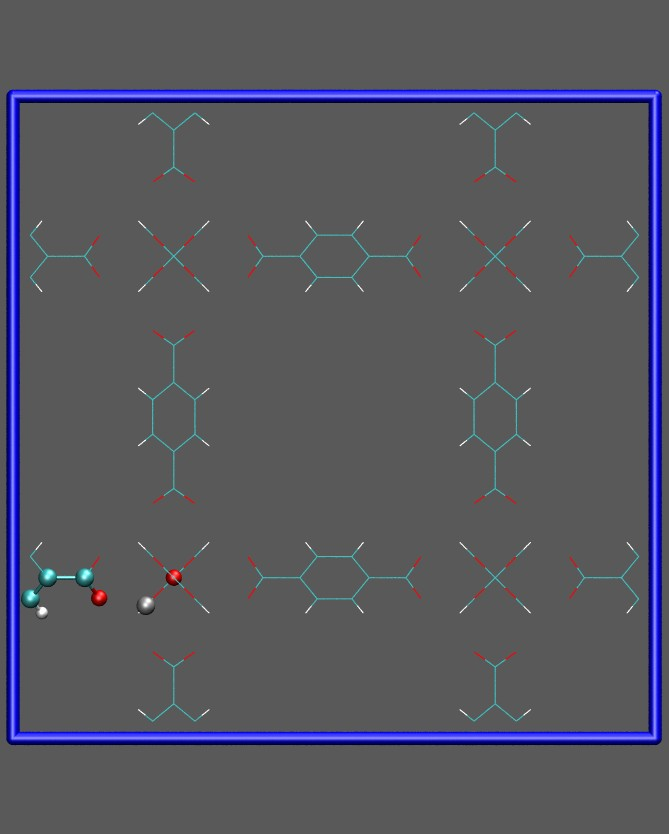
\includegraphics[width=7.5cm]{./InputFiles/IRMOF-1-asymmetric.jpg}}
   \subfloat[The full unit cell of IRMOF-1 has 424 atoms.]{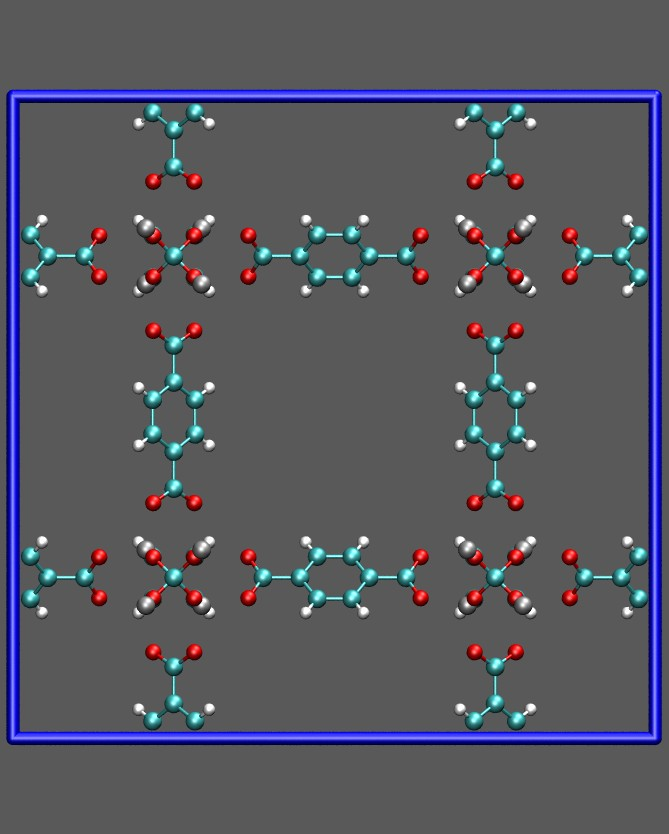
\includegraphics[width=7.5cm]{./InputFiles/IRMOF-1.jpg}}
  \caption{Asymmetric unit cells: the left figure shows the seven crystallographicly different atoms in the IRMOF-1 structure in
           ball-and-stick format. The `copies' (crystallographically identical atoms) are shown as lines. The right figure
           shows the full unit cell of IRMOF-1 in ball-and-stick.}
  \label{Fig: asymmetric}
\end{figure}

RASPA can then be run using:
\begin{verbatim}
    SimulationType       MonteCarlo
    NumberOfCycles       0
    InitializationCycles 0

    Forcefield           GenericMOFs

    Framework     0
    FrameworkName IRMOF-1
    UnitCells     1 1 1
\end{verbatim}
and in the directory \verb=`Movies/System_0/i'= several files appear: 
\begin{itemize}
\item{\verb=`Framework_0_initial_1_1_1.cif'=}\\
The framework in CIF-format at the start of the simulation.
\item{\verb=`Framework_0_initial_1_1_1_P1.cif'=}\\
The framework in CIF-format at the start of the simulation converted to P1 (no symmetry).
\item{\verb=`Framework_0_initial.pdb'=}\\
The framework in PDB-format at the start of the simulation converted to P1 (no symmetry).
\end{itemize}
The files named `final' are the structures at the end of the simulation. There are several programs that can read and view CIF-files:
e.g. Jmol (free), Mercury (free), Crystal Maker (commercial, free demo), Materials Studio (commercial), and Gaussview (commercial).
The PDB-files can be viewed in the freely available VMD-program.
\begin{center}
\shadowbox{
\begin{minipage}{\linewidth}
 Tip: always double check the \verb=`Framework_0_initial_1_1_1_P1.cif'=, if you see something strange then check 
  \verb=`_symmetry_space_group_name_Hall'= and the fractional positions.
\end{minipage}}
\end{center}


Space group 225 has 192 elements and the first 10 elements look like (see the file `src/spacegroup.c' for the complete set):
\begin{align*}
  x'&=x  \qquad &y'&=y   \qquad &z'&=z\\
  x'&=-x \qquad &y'&=-y  \qquad &z'&=z\\
  x'&=-x \qquad &y'&=y   \qquad &z'&=-z\\
  x'&=x  \qquad &y'&=-y  \qquad &z'&=-z\\
  x'&=z  \qquad &y'&=x   \qquad &z'&=y\\
  x'&=z  \qquad &y'&=-x  \qquad &z'&=-y\\
  x'&=-z \qquad &y'&=-x  \qquad &z'&=y\\
  x'&=-z \qquad &y'&=x   \qquad &z'&=-y\\
  x'&=y; \qquad &y'&=z   \qquad &z'&=x\\
  x'&=-y \qquad &y'&=z   \qquad &z'&=-x\\
  x'&=y  \qquad &y'&=-z  \qquad &z'&=-x\\
  \dots
\end{align*}
The procedure to generate a unit cell is to loop over the elements of the spacegroup and the atoms in the asymmetric unit cell, and to
apply simply all the rule. For each new $x',y',z'$ position a check is needed whether the same position has already been added
(doubles have to be removed). After this procedure the 7 positions have been expanded to 424 positions. The fractional positions
are transformed in the final step to Cartesian positions.



\subsection{Fractional occupancies in zeolites}

The procedure from asymmetric to full unit cell is rather simple when the fractional occupancies are unity. However, quite often there
is some disorder the type of atoms. For example, in zeolites like FAU the Si/Al ratio is specified, but it is unknown where the aluminum
actually is. Zeolite X is faujasite with a high amount of aluminum. The FAU structure with a Si/Al ratio of unity is given by
\begin{verbatim}
     data_NaX
     
     _audit_creation_method RASPA-1.0
     _audit_creation_date 2011-2-20
     _audit_author_name 'David Dubbeldam'
     
     _cell_length_a    25.099
     _cell_length_b    25.099
     _cell_length_c    25.099
     _cell_angle_alpha 90
     _cell_angle_beta  90
     _cell_angle_gamma 90
     _cell_volume      14273.9
     
     _symmetry_cell_setting          cubic
     _symmetry_space_group_name_Hall '-F 2uv 2vw 3'
     _symmetry_space_group_name_H-M  'F d -3'
     _symmetry_Int_Tables_number     203
     
     loop_
     _atom_site_label
     _atom_site_type_symbol
     _atom_site_fract_x
     _atom_site_fract_y
     _atom_site_fract_z
     Si1      Si4+  -0.05381   0.12565   0.03508
     Al1      Al3+  -0.05524   0.03639   0.12418
     O1       O2-   -0.1099    0.0003    0.1056 
     O2       O2-   -0.0011   -0.0028    0.1416 
     O3       O2-   -0.0346    0.0758    0.0711 
     O4       O2-   -0.0693    0.0726    0.18   
\end{verbatim}
Now the aluminum and silicon are alternating and L\"owestein rule is obeyed. For higher Si/Al ratios
the `Al' position is fractionally occupied and a certain percentage might actually be silicon. The
procedure here is to first generate the full unit cell of FAU with 96 aluminum (the maximum amount)
and judiciously replace aluminum by silicon in the full unit cell.

\begin{verbatim}
     SimulationType                MC
     NumberOfCycles                0
     NumberOfInitializationCycles  0
     PrintEvery                    10
     
     Forcefield                    Local
     
     Substitute 0 Al1 Si1
     Substitute 5 Al1 Si1
     Substitute 10 Al1 Si1
     Substitute 15 Al1 Si1
     Substitute 20 Al1 Si1
     RandomlySubstitute 75 Al1 Si1
     
     Framework 0
     FrameworkName NaX
     UnitCells 1 1 1
     ExternalTemperature 300.0
\end{verbatim}

It reads the CIF-file which is Nax with 96 aluminum. You can use two types of commands to replace an atom:
\begin{itemize}
\item{Substitute}\\
For example. \verb=Substitute 10 Al1 Si1= means replace the 10th \verb=Al1= by \verb=Si1=.
\item{RandomlySubstitute}\\
For example, \verb=RandomlySubstitute 75 Al1 Si1= means randomly substitute 75 \verb=Al1= by \verb=Si1=.
\end{itemize}

When you do them both, first the fixed rules are substituted and next the random ones with the `leftovers'.
The first one `Substitute' is useful to always have the same structure. You could make a random structure once, look in the output which Al was substituted and use the next time the `Substitute' command.
In this way, you always work with the spacegroup NaX structure (not in P1) which is afterwards change by specifying rules.

More problematic are when several atoms have fractional occupancies lower than unity. Consider IRMOF-8 shown in Fig. \ref{Fig: IRMOF-8}.
The linker molecules are disordered over two possible positions. One of these needs to be selected per linker. First the unit cell
is generated from the asymmetric unit cell and subsequently the unit cell needs to be edited. Program which can do just that are
Materials Studio, Gaussview, etc. After the cell has been created and edited, the file needs to be placed
in `structures/mofs/cif'. Structures with disorder needs to be created at unit cell level (P1).

Even more difficult is MOF-{\bf 1}. Here the cif-file also contains several possibilities, but is not a priori known which ones to choose, i.e.
what is the structure of the Dabco unit (1,4-diazabicyclo[2.2.2]octane) within the framework? One possibility is to choose a structure
and use a quantum code and minimize the periodic unit cell. The result is shown in Fig. \ref{Fig: cif vs dmol}.

Note that all these procedures are necessary, but it is still an open question, especially for MOFs, whether you can keep the framework rigid or not.
However, it is very hard to calibrate a flexible framework model and for this a substantial amount of reliable experimental data is required.

\subsection{Format of the framework atoms}

The atom-types in CIF-files are constructed from the name of the element and an identifier, e.g.\ \verb=`C10'= carbon type 10.
Usually these carbon atoms are different because they have either different charges or different Van der Waals parameters.

Sometimes a force field is defined to have interactions on an atom-type which depends on its neighbors. For example, the oxygen atom is different
whether it is connected to a silicon or to an aluminum atom. Therefore the atom are labelled using
\begin{verbatim}
ModifyFrameworkAtomConnectedTo O1 Oa1 Al1
ModifyFrameworkAtomConnectedTo O2 Oa2 Al1
ModifyFrameworkAtomConnectedTo O3 Oa3 Al1
ModifyFrameworkAtomConnectedTo O4 Oa4 Al1
\end{verbatim}
which modifies \verb=`O1'= to \verb=zOa1'= when connected to \verb=`Al1'=, etc.
In the CIF-file you can list the new framework atom with unknown position \verb=`?'=.
\begin{verbatim}
     loop_
     _atom_site_label
     _atom_site_type_symbol
     _atom_site_fract_x
     _atom_site_fract_y
     _atom_site_fract_z
     Si1      Si4+  -0.05381   0.12565   0.03508
     Al1      Al3+  -0.05524   0.03639   0.12418
     O1       O2-   -0.1099    0.0003    0.1056 
     O2       O2-   -0.0011   -0.0028    0.1416 
     O3       O2-   -0.0346    0.0758    0.0711 
     O4       O2-   -0.0693    0.0726    0.18   
     Oa1      O2-    ?         ?         ?      
     Oa2      O2-    ?         ?         ?      
     Oa3      O2-    ?         ?         ?      
     Oa4      O2-    ?         ?         ?      
\end{verbatim}
Alternatively, you can list the atom types \verb=`Oa1'=--\verb=`Oa4'= in your \verb=`pseudo_atoms.def'= file.

Other times a force field is defined as
\begin{verbatim}
     # rules to overwrite
     0
     # number of defined interactions
     4
     # type      type2       interaction
     O           O           lennard-jones     29.4338257        3.062219744
     O           Si          lennard-jones     49.05711264       3.483346249
     Si          Si          lennard-jones     81.76308187       3.962387454
     CH4_sp3     O           lennard-jones    115.00             3.47
     # mixing rules to overwrite
     0
\end{verbatim}
Here, we have that all oxygens in the framework are of the same type, and all silicon is of the same type.
In this case, we would like to map \verb=`O1'=, \verb=`O2'=, \verb=`O3'=, etc.\ to \verb=`O'=,
and \verb=`Si1'=, \verb=`Si2'=, etc.\ to \verb=`Si'=.
You can acgieve this using
\begin{verbatim}
     RemoveAtomNumberCodeFromLabel yes
\end{verbatim}

Suppose you want to use MFI with only \verb=`O'= and \verb=`Si'=. MFI is defined using 
\begin{verbatim}
     Si1      Si4+   0.42238   0.0565   -0.33598
     Si2      Si4+   0.30716   0.02772  -0.1893 
     \dots
     O1       O2-    0.3726    0.0534   -0.2442 
     O2       O2-    0.3084    0.0587   -0.0789 
     \dots
\end{verbatim}


The force field in \verb=`force_field.def'=
\begin{verbatim}
     # rules to overwrite
     0
     # number of defined interactions
     1
     # type      type2       interaction
     CH4_sp3     O           lennard-jones    115.00          3.47
     # mixing rules to overwrite
     0
\end{verbatim}
The \verb=`pseudo_atom.def'=
\begin{scriptsize}
\begin{verbatim}
     #number of pseudo atoms
     3
     #type      print   as  scatt mass       charge  polarization B-factor radii   connectivity  anisotropic anisotropic-type   tinker-type
     O          yes      O     O  15.9994   -1.025   0.0          1.0      0.5     2             0           absolute           0
     Si         yes     Si    Si  28.0855    2.05    0.0          1.0      1.18    4             0           absolute           0
     CH4_sp3    yes      C     C  16.04246   0.0     0.0          1.0      1.00    0             0           absolute           0
\end{verbatim}
\end{scriptsize}
and the output file will show:
\begin{scriptsize}
\begin{verbatim}
     Pseudo atoms: 2
     ===========================================================================
     Pseudo Atom[   0] Name Si       Oxydation:          Element: Si4+ pdb-name: Si   Scat. Types: 111  14 Mass=28.085498706 B-factor:0.000
                      Charge=2.050     Polarization=0.017    [A^3] (considered a charged atom and no polarization)  Interactions:  no
                      Anisotropic factor:    0.000 [-] (Absolute), Radius:    1.110 [A]
     Pseudo Atom[   1] Name O        Oxydation:          Element: O2-  pdb-name: O    Scat. Types: 105   8 Mass=15.999404927 B-factor:0.000
                      Charge=-1.025    Polarization=3.880    [A^3] (considered a charged atom and no polarization)  Interactions:  no
                      Anisotropic factor:    0.000 [-] (Absolute), Radius:    0.660 [A]
\end{verbatim}
\end{scriptsize}


\begin{figure}[p]
  \centering
   \subfloat[The IRMOF-8 structure as directly computed from the asymmetric positions and the space group.]{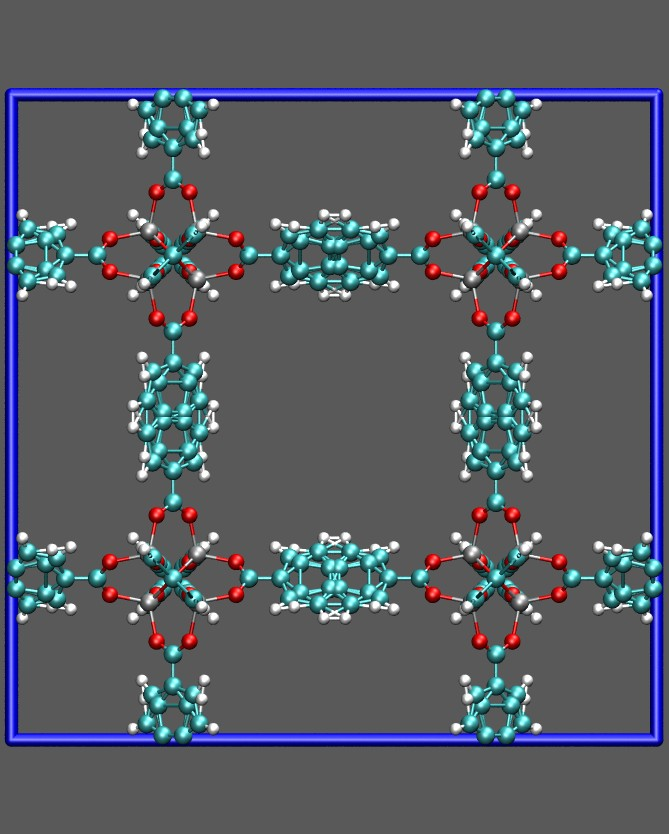
\includegraphics[width=6.0cm]{./InputFiles/IRMOF-8-full.jpg}}
   \hskip 1cm
   \subfloat[The IRMOF-8 after making a selection, shown is only one of the possibilities.]{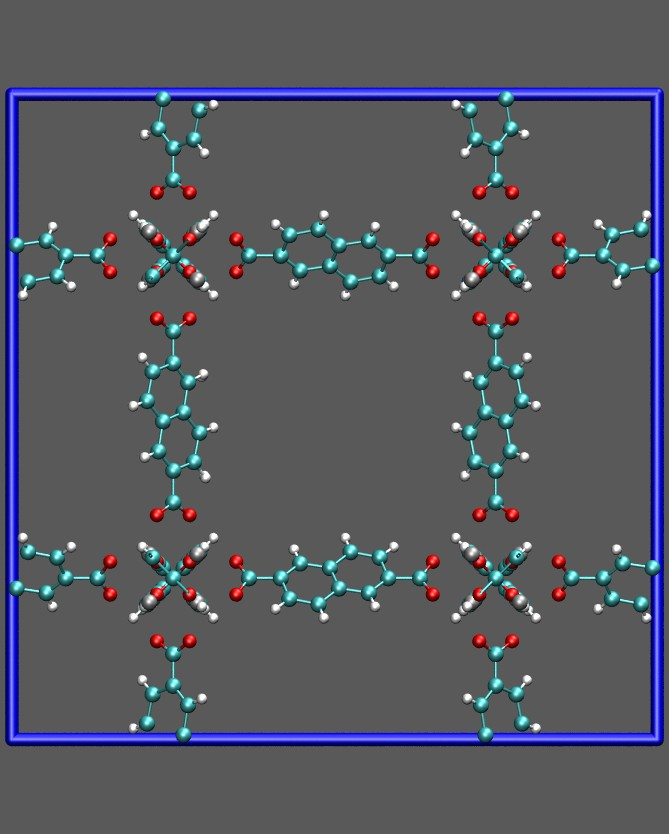
\includegraphics[width=6.0cm]{./InputFiles/IRMOF-8.jpg}}
  \caption{IRMOF-8 has linkers which are disordered, the linker atoms have a fractional occupancy of 0.5, The atoms however are not individually disorder and
           there are two disordered linker, one out of two possibilities needs to be selected per linker position.}
  \label{Fig: IRMOF-8}
  \centering
   \subfloat[The MOF-{\bf 1} structure from the cif-file.]{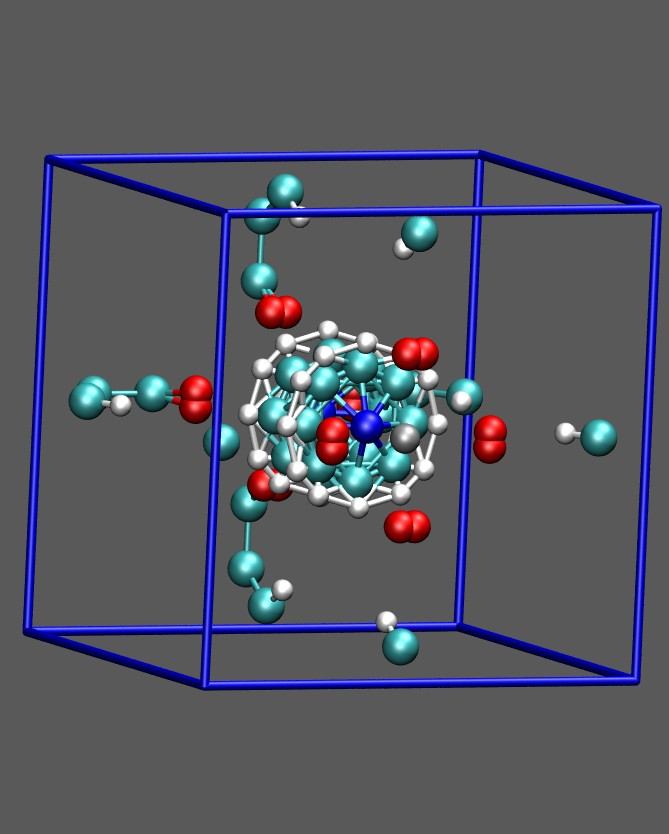
\includegraphics[width=6.0cm]{./InputFiles/MOF-1-cif.jpg}}
   \hskip 1cm
   \subfloat[The MOF-{\bf 1} structure edited and optimized with the quantum program dmol
                            (plane wave code).]{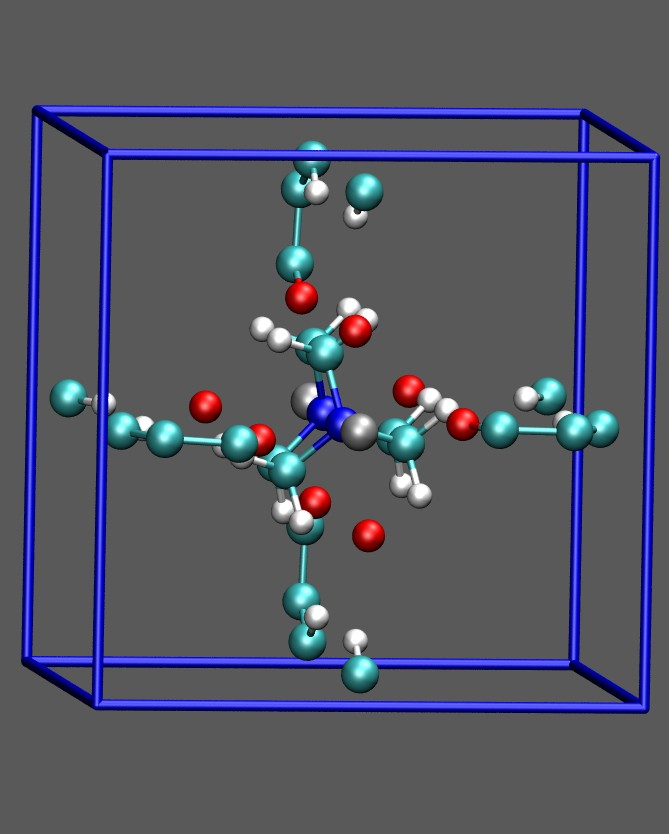
\includegraphics[width=6.0cm]{./InputFiles/MOF-1-dmol.jpg}}
  \caption{The MOF-1 structure is synthesized as [Zn$_2$(1,4-bdc)2(Dabco)]. The Dabco (1,4-diazabicyclo[2.2.2]octane) is very
          disordered with occupancies of 0.38 for the carbon and 0.5 for the hydrogen. The cif-file shown on the left shows all
          possibilities on top of each other. Here, just choosing one of the possibilities
          is difficult and it is not obvious which atoms to select. The brute force method is to select one possible choice and
          use a quantum plane wave for periodic structures and optimize the full unit cell. In this case it is feasible because
          of the low amount of atoms in the unit cell (only 54 atoms).}
  \label{Fig: cif vs dmol}
\end{figure}

\subsection{Typing the atoms of the framework}

Atoms from a pdb- or cif-file are usually labeled e.g. `C' for a carbon atom. In many force fields different carbon types have different charges.
It is necessary to `type' the structure and RASPA contains tools to do this. Let's assume the original structure always contains elements like `H', `C',
`N', `O', etc. and we want to type them `Mof\_Ha', `Mof\_Hb', etc. A force field type called `Typing' preexists. It only defines the `pseudo\_atoms.def' file:
\begin{small}
\begin{verbatim}
     #number of pseudo atoms
     43
     #type      print   as  scat     mass       charge    polarization B-factor radii  connectivity
     UNIT       no      H      H     1.0        1.0       0.0          1.0      1.0    0
     He         yes     He     He    4.002602   0.0       0.0          1.0      1.0    0
     Zn         yes     Zn1    Zn    65.37      0.0       0.0          1.0      1.448  0
     Zn1        yes     Zn1    Zn    65.37      0.0       0.0          1.0      1.448  0
     Cu         yes     Cu1    Cu    63.546     0.0       0.0          1.0      1.4    0
     Cu1        yes     Cu1    Cu    63.546     0.0       0.0          1.0      1.4    0
     O          yes     O      O     15.9994    0.0       0.0          1.0      0.68   2
     O1         yes     O1     O     15.9994    0.0       0.0          1.0      0.68   2
     O2         yes     O2     O     15.9994    0.0       0.0          1.0      0.68   2
     O3         yes     O3     O     15.9994    0.0       0.0          1.0      0.68   2
     O4         yes     O4     O     15.9994    0.0       0.0          1.0      0.68   2
     C          yes     C      C     12.0107    0.0       0.0          1.0      0.720  0
     C1         yes     C1     C     12.0107    0.0       0.0          1.0      0.720  0
     C2         yes     C2     C     12.0107    0.0       0.0          1.0      0.720  0
     C3         yes     C3     C     12.0107    0.0       0.0          1.0      0.720  0
     C4         yes     C4     C     12.0107    0.0       0.0          1.0      0.720  0
     C5         yes     C5     C     12.0107    0.0       0.0          1.0      0.720  0
     C6         yes     C6     C     12.0107    0.0       0.0          1.0      0.720  0
     C7         yes     C7     C     12.0107    0.0       0.0          1.0      0.720  0
     C8         yes     C8     C     12.0107    0.0       0.0          1.0      0.720  0
     C9         yes     C9     C     12.0107    0.0       0.0          1.0      0.720  0
     C10        yes     C10    C     12.0107    0.0       0.0          1.0      0.720  0
     C11        yes     C11    C     12.0107    0.0       0.0          1.0      0.720  0
     C12        yes     C12    C     12.0107    0.0       0.0          1.0      0.720  0
     C13        yes     C13    C     12.0107    0.0       0.0          1.0      0.720  0
     C14        yes     C14    C     12.0107    0.0       0.0          1.0      0.720  0
     C15        yes     C15    C     12.0107    0.0       0.0          1.0      0.720  0
     C16        yes     C16    C     12.0107    0.0       0.0          1.0      0.720  0
     N          yes     N      N     14.00674   0.0       0.0          1.0      0.68   0
     N1         yes     N1     N     14.00674   0.0       0.0          1.0      0.68   0
     N2         yes     N2     N     14.00674   0.0       0.0          1.0      0.68   0
     N3         yes     N3     N     14.00674   0.0       0.0          1.0      0.68   0
     N4         yes     N4     N     14.00674   0.0       0.0          1.0      0.68   0
     H          yes     H      H     1.00794    0.0       0.0          1.0      0.320  0
     H1         yes     H1     H     1.00794    0.0       0.0          1.0      0.320  0
     H2         yes     H2     H     1.00794    0.0       0.0          1.0      0.320  0
     H3         yes     H3     H     1.00794    0.0       0.0          1.0      0.320  0
     H4         yes     H4     H     1.00794    0.0       0.0          1.0      0.320  0
     H5         yes     H5     H     1.00794    0.0       0.0          1.0      0.320  0
     H6         yes     H6     H     1.00794    0.0       0.0          1.0      0.320  0
     H7         yes     H7     H     1.00794    0.0       0.0          1.0      0.320  0
     H8         yes     H8     H     1.00794    0.0       0.0          1.0      0.320  0
     H9         yes     H9     H     1.00794    0.0       0.0          1.0      0.320  0
\end{verbatim}
\end{small}

As an example, let's type the structure `NU-100' \cite{Farha2010}. Figure \ref{Fig: NU-100 cluster} shows the NU-100 cluster with linkers and
metal-corners. The pictures shows the different types of atoms and has been used to compute CHelpG charges.
In the RASPA input-file you can use the typing command:
\begin{verbatim}
ModifyFrameworkAtomConnectedTo C Mof_Ca O
\end{verbatim}
Look for a `C' atom, check if it is connect to an `O' atom and if so, type it `Mof\_Ca'.
It is also possible to define two neighbors:
\begin{verbatim}
ModifyFrameworkAtomConnectedTo C Mof_Cc Mof_Cb Mof_Cb
\end{verbatim}
Look for an `C' atom, if it is connect to a `Mof\_Cb' and to another `Mof\_Cb' atom, then type is `Mof\_Cc'.

\begin{figure}[t]
  \centering
   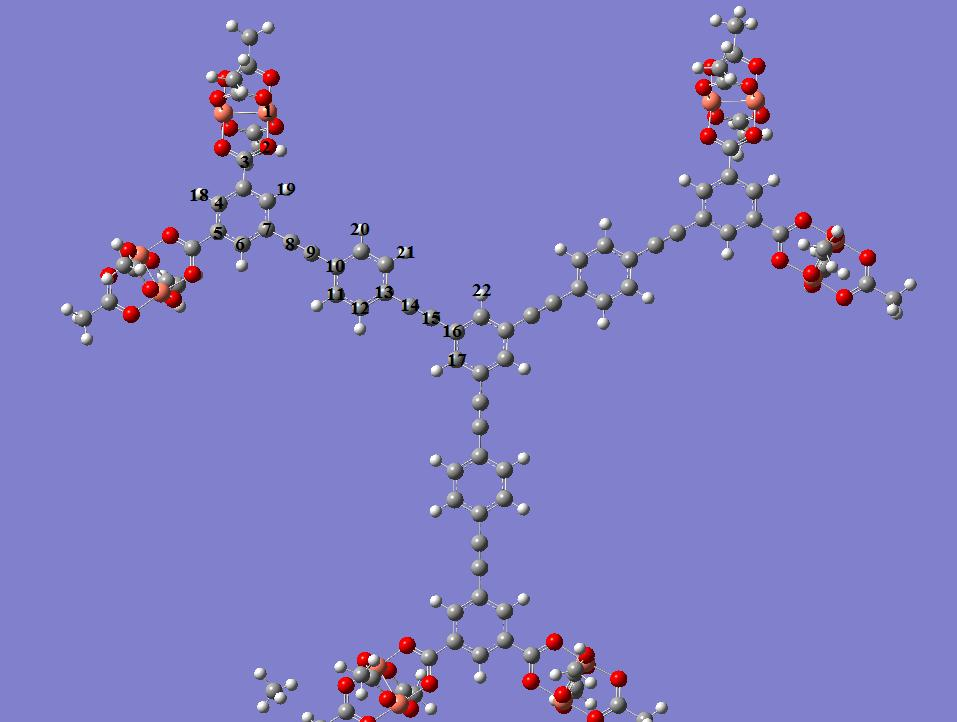
\includegraphics[width=15cm]{./InputFiles/NU-100.jpg}
  \caption{Cluster used for deriving partial charges on atoms in NU-100SP \cite{Farha2010}.}
  \label{Fig: NU-100 cluster}
\end{figure}


The input-file to type `NU-100' is
\begin{verbatim}
     SimulationType                   MC
     NumberOfCycles                   0
     
     Forcefield                       Local
     
     Framework 0
     FrameworkName NU-100SP
     UnitCells 1 1 1
     InputFileType cssr
     ExternalTemperature 298.0
     
     ModifyFrameworkAtomConnectedTo C C1 O
     ModifyFrameworkAtomConnectedTo C C2 C1
     ModifyFrameworkAtomConnectedTo C C3 C2 C2
     ModifyFrameworkAtomConnectedTo C C4 C2
     ModifyFrameworkAtomConnectedTo C C5 C4
     ModifyFrameworkAtomConnectedTo C C6 C5
     ModifyFrameworkAtomConnectedTo C C7 C6
     ModifyFrameworkAtomConnectedTo C C8 C7
     ModifyFrameworkAtomConnectedTo C C9 C8
     ModifyFrameworkAtomConnectedTo C C10 C9
     ModifyFrameworkAtomConnectedTo C C11 C10
     ModifyFrameworkAtomConnectedTo C C12 C11
     ModifyFrameworkAtomConnectedTo C C13 C12
     ModifyFrameworkAtomConnectedTo C C14 C13
     ModifyFrameworkAtomConnectedTo C C15 C14
     ModifyFrameworkAtomConnectedTo H H1 C3
     ModifyFrameworkAtomConnectedTo H H2 C4
     ModifyFrameworkAtomConnectedTo H H3 C9
     ModifyFrameworkAtomConnectedTo H H4 C10
     ModifyFrameworkAtomConnectedTo H H5 C15
     ModifyFrameworkAtomConnectedTo O O2 C1
     ModifyFrameworkAtomConnectedTo Cu Cu O2
\end{verbatim}

For MOFs, the easiest start-point to type is the carboxylate group. The carbon connected to the oxygen is typed `Mof\_Ca', the carbon
connected to `Mof\_Cb' is typed `Mof\_Cc'. The third line is important: the carbon should only be typed `Mof\_Cc' when it is connected
to an `Mof\_Cb' and another `Mof\_Cb'. This must be done like this, otherwise the atom which is above called `Mof\_Cd' would also
be wrongly labeled `Mof\_Cc'. After running RASPA, the `Movie'-directory contains the file `Framework\_intitial.cssr' which is the
cssr-file with complete typing. This file can be copied to `structures/mofs/cssr' and given an appropriate name.
Each pseudatom type can now be assigned a different charge in the `psuedo\_atoms.def' file of the 
`NU-100' forcefield.

Note that the lines containing the typing-rules  are performed top to bottom and in later rules one can use the new names of the previous rules.


\section{Using CIF-files}

\subsection{Definition of CIF-files}

CIF files present crystallographic data in an human readable free format. Let's look at an example:

\begin{footnotesize}
\begin{verbatim}
data_FAU_SI

_audit_creation_method RASPA-1.0
_audit_creation_date 2011-2-19
_audit_author_name 'David Dubbeldam'

_citation_author_name        'J.J. Hriljac, M.M. Eddy, A.K. Cheetham, J.A. Donohue,  and G.J. Ray'
_citation_title              'Powder Neutron Diffraction and Si-29 MAS NMR Studies of Siliceous Zeolite-Y'
_citation_journal_abbrev     'J. Solid State Chem.'
_citation_journal_volume     106
_citation_page_first         66
_citation_page_last          72
_citation_year               1993

_cell_length_a    24.2576
_cell_length_b    24.2576
_cell_length_c    24.2576
_cell_angle_alpha 90
_cell_angle_beta  90
_cell_angle_gamma 90
_cell_volume      14273.9

_symmetry_cell_setting          cubic
_symmetry_space_group_name_Hall '-F 4vw 2vw 3'
_symmetry_space_group_name_H-M  'F d -3 m'
_symmetry_Int_Tables_number     227

loop_
_symmetry_equiv_pos_as_xyz
 'x,y,z'
 '-x+3/4,-y+1/4,z+1/2'
  ................
  ................
  ................
 'z,-y+3/4,-x+3/4'
 'z+1/2,y+1/2,x'

loop_
_atom_site_label
_atom_site_type_symbol
_atom_site_fract_x
_atom_site_fract_y
_atom_site_fract_z
_atom_site_charge
_atom_site_polarization
Si1      Si4+  -0.05392   0.1253    0.03589   2.05    0
O1       O2-    0        -0.10623   0.10623  -1.025   0
O2       O2-   -0.00323  -0.00323   0.14066  -1.025   0
O3       O2-    0.0757    0.0757   -0.03577  -1.025   0
O4       O2-    0.07063   0.07063   0.32115  -1.025   0
\end{verbatim}
\end{footnotesize}

The `data\_' string signal the start of a data block. Each data block corresponds to a different structures, and typically only one structure is present (although it
possible to combine more than one structure in a single file).
The CIF instructions are divided into \emph{data name categories}, such as `\_atom\_site\_' to describe atomic site parameters, `\_cell\_'
to describe the cell parameters, `\_symmetry\_' to specify  space group symmetry, etc.
CIF data names begin with an underscore. For some data name the data can be provided using a list of data items. Such data items are preceded by a `loop\_' string.
The `\_atom\_site\_' section is typical example. The order of the data items correspond to the order in which the actual data is provided.

A nice feature of CIFs is that one can easily extend the syntax to include nom-standard data item. For example. in the `\_atom\_site\_' section,
the data items `\_atom\_site\_label', `\_atom\_site\_type\_symbol', `\_atom\_site\_fract\_x', `\_atom\_site\_fract\_y', `\_atom\_site\_charge' belong to the official CIF specification,
but `\_atom\_site\_charge', `\_atom\_site\_polarization', `\_atom\_site\_anisotropic\_displacement', `\_atom\_site\_anisotropic\_type',
and `\_atom\_site\_print\_to\_pdb' have been added in RASPA CIFs. Used in this fashion, they provide a replacement for the `pseudo\_atoms.def' file.
Note that if a `pseudo\_atoms.def' file is used, the value in that file will have preference over the CIF-file values (if they both define the same atom-type).

\subsection{What charge definition is used? `pseudo\_atom.def' or from the CIF-file?}

For adsorbates the charges are defined via the atom-type in the `pseudo\_atom.def' file.
For the framework, there are several scenarios:
\begin{itemize}
\item{define charges via the CIF-file}\\
If you want a possibly different charge for each atom, then use the option:
\begin{verbatim}
  UseChargesFromCIFFile yes
\end{verbatim}
and define the charge using the field `\_atom\_site\_charge' in the CIF-file.
Atom-types from the CIF-file that are not defined in the `pseudo\_atom.def' are automatically added, atoms that are already defined as a type in
the `pseudo\_atom.def' get the charge from the CIF-file. In the output-file in the list of pseudo-atoms you will see e.g.
\begin{verbatim}
  Charge=0.111115012    (av)
\end{verbatim}
which signals that for this atom-type the averages charge is listed (because each atom potentially can have a different value in this case).
This is a typical case for simulations based on CHelpG charges from quantum.
\item{define charges via the `pseudo\_atom.def' file}\\
If you want the same charge for all atoms of the atom-type, then you can list all of these in the `pseudo\_atom.def' file and use
\begin{verbatim}
  UseChargesFromCIFFile no
\end{verbatim}
which is the default. Any atoms with a type known in the CIF-file will get a charge given in the `pseudo\_atom.def' file; atoms of unknown type
will be added to the pseudo-atoms but with a charge of zero. The latter is probably not what you want, so make sure you have listed all atom type in `pseudo\_atom.def' file.
\item{Define charges using `Charge Equilibration'}\\
No matter what you define in the `pseudo\_atom.def' or CIF-file, the charges will be recompute using the charge-equilbration scheme of Wilmer and Snurr.
\end{itemize}

\begin{center}
\begin{shadedbox}
Tip: the charges that are actually used in the simulation are listed as the column `\_atom\_site\_charge'
in the file `Movies/System\_0/Framework\_0\_initial\_P1.cif'.
 Also, check the ouput-file for the net-charge of the framework, and the smallest and largest charge it found, e.g.\
           \begin{verbatim}
             Framework has net charge: 0.000000
             largest charge : 0.931455
             smallest charge: -0.626799
           \end{verbatim}
\end{shadedbox}
\end{center}

\subsection{How to choose atom-types?}

The FAU structure above was defined with atom types: `Si1', `O1', `O2', `O3', and `O4'. Using the option:
\begin{verbatim}
  RemoveAtomNumberCodeFromLabel yes
\end{verbatim}
these 5 types will be reduces to 2: `Si' and `O'. There are advantages and disadvantages to each of the options:
\begin{itemize}
\item{Specific types}\\
  Use if
  \begin{enumerate}
    \item{You want RDF between the adsorbate atoms and the specific framework atoms.}   
    \item{If you have different VDW parameters for each specific framework atom (so `O1', `O2', `O3', `O4' would have different VDW parameters).}
  \end{enumerate}
\item{Reduced types}\\
  Use if you are not interested in the difference between `O1', \dots, `O4', but only have a single VDW parameter set for that atom type `O'.
  Note: you can still list different charges for each of these atoms in the CIF-file.
  This options avoid excessive number of pseudo-atoms, which can clutter the output, and avoids having lots of different RDFs (and manually having to averages these afterwards).
\end{itemize}


\newpage
\clearpage
\subsection*{Appendix: space group information}

\begin{center}
\begin{small}
\begin{longtable}{|l|l|l|l|l|l|l|l|l|l|l|}
\hline
\multicolumn{10}{|>{\columncolor{orange-red}}c|}{triclinic}\\
\hline
\rowcolor{niceyellow}
id & Int. Nr. & long Hermann-    & Hall name & cell choice & centered &\# & Chiral & Centric & Enantio-\\
\rowcolor{niceyellow}
   &          & Mauguin name     &           &             &          &   &        &         & morphic\\
\hline
1 &1 &P 1 &P 1 &cell choice 1 &primitive &1 &yes &no &no \\ 
2 &2 &P -1 &-P 1 &cell choice 1 &primitive &2 &yes &no &no \\ 
\hline
\caption{Triclinic spacegroup information.}
\end{longtable}


\begin{longtable}{|l|l|l|l|l|l|l|l|l|l|l|}
\hline
\multicolumn{10}{|>{\columncolor{orange-red}}c|}{monoclinic}\\
\hline
\rowcolor{niceyellow}
id & Int. Nr. & long Hermann-    & Hall name & cell choice & centered &\# & Chiral & Centric & Enantio-\\
\rowcolor{niceyellow}
   &          & Mauguin name     &           &             &          &   &        &         & morphic\\
\hline
3 &3 &P 1 2 1 &P 2y &unique axis b &primitive &2 &no &yes &no \\ 
4 &3 &P 1 1 2 &P 2 &unique axis c &primitive &2 &no &yes &no \\ 
5 &3 &P 2 1 1 &P 2x &unique axis a &primitive &2 &no &yes &no \\ 
6 &4 &P 1 21 1 &P 2yb &unique axis b &primitive &2 &no &yes &no \\ 
7 &4 &P 1 1 21 &P 2c &unique axis c &primitive &2 &no &yes &no \\ 
8 &4 &P 21 1 1 &P 2xa &unique axis a &primitive &2 &no &yes &no \\ 
9 &5 &C 1 2 1 &C 2y &b, cell choice 1 &c &4 &no &yes &no \\ 
10 &5 &A 1 2 1 &A 2y &b, cell choice 2 &a &4 &no &yes &no \\ 
11 &5 &I 1 2 1 &I 2y &b, cell choice 3 &body &4 &no &yes &no \\ 
12 &5 &A 1 1 2 &A 2 &c, cell choice 1 &a &4 &no &yes &no \\ 
13 &5 &B 1 1 2 &B 2 &c, cell choice 2 &b &4 &no &yes &no \\ 
14 &5 &I 1 1 2 &I 2 &c, cell choice 3 &body &4 &no &yes &no \\ 
15 &5 &B 2 1 1 &B 2x &a, cell choice 1 &b &4 &no &yes &no \\ 
16 &5 &C 2 1 1 &C 2x &a, cell choice 2 &c &4 &no &yes &no \\ 
17 &5 &I 2 1 1 &I 2x &a, cell choice 3 &body &4 &no &yes &no \\ 
18 &6 &P 1 m 1 &P -2y &unique axis b &primitive &2 &no &no &no \\ 
19 &6 &P 1 1 m &P -2 &unique axis c &primitive &2 &no &no &no \\ 
20 &6 &P m 1 1 &P -2x &unique axis a &primitive &2 &no &no &no \\ 
21 &7 &P 1 c 1 &P -2yc &b, cell choice 1 &primitive &2 &no &no &no \\ 
22 &7 &P 1 n 1 &P -2yac &b, cell choice 2 &primitive &2 &no &no &no \\ 
23 &7 &P 1 a 1 &P -2ya &b, cell choice 3 &primitive &2 &no &no &no \\ 
24 &7 &P 1 1 a &P -2a &c, cell choice 1 &primitive &2 &no &no &no \\ 
25 &7 &P 1 1 n &P -2ab &c, cell choice 2 &primitive &2 &no &no &no \\ 
26 &7 &P 1 1 b &P -2b &c, cell choice 3 &primitive &2 &no &no &no \\ 
27 &7 &P b 1 1 &P -2xb &a, cell choice 1 &primitive &2 &no &no &no \\ 
28 &7 &P n 1 1 &P -2xbc &a, cell choice 2 &primitive &2 &no &no &no \\ 
29 &7 &P c 1 1 &P -2xc &a, cell choice 3 &primitive &2 &no &no &no \\ 
30 &8 &C 1 m 1 &C -2y &b, cell choice 1 &c &4 &no &no &no \\ 
31 &8 &A 1 m 1 &A -2y &b, cell choice 2 &a &4 &no &no &no \\ 
32 &8 &I 1 m 1 &I -2y &b, cell choice 3 &body &4 &no &no &no \\ 
33 &8 &A 1 1 m &A -2 &c, cell choice 1 &a &4 &no &no &no \\ 
34 &8 &B 1 1 m &B -2 &c, cell choice 2 &b &4 &no &no &no \\ 
35 &8 &I 1 1 m &I -2 &c, cell choice 3 &body &4 &no &no &no \\ 
36 &8 &B m 1 1 &B -2x &a, cell choice 1 &b &4 &no &no &no \\ 
37 &8 &B m 1 1 &C -2x &a, cell choice 2 &c &4 &no &no &no \\ 
38 &8 &I m 1 1 &I -2x &a, cell choice 3 &body &4 &no &no &no \\ 
39 &9 &C 1 c 1 &C -2yc &b, cell choice 1 &c &4 &no &no &no \\ 
40 &9 &A 1 n 1 &A -2yab &b, cell choice 2 &a &4 &no &no &no \\ 
41 &9 &I 1 a 1 &I -2ya &b, cell choice 3 &body &4 &no &no &no \\ 
42 &9 &A 1 a 1 &A -2ya &-b, cell choice 1 &a &4 &no &no &no \\ 
43 &9 &C 1 n 1 &C -2yac &-b, cell choice 2 &c &4 &no &no &no \\ 
44 &9 &I 1 c 1 &I -2yc &-b, cell choice 3 &body &4 &no &no &no \\ 
45 &9 &A 1 1 a &A -2a &c, cell choice 1 &a &4 &no &no &no \\ 
46 &9 &B 1 1 n &B -2ab &c, cell choice 2 &b &4 &no &no &no \\ 
47 &9 &I 1 1 b &I -2b &c, cell choice 3 &body &4 &no &no &no \\ 
48 &9 &B 1 1 b &B -2b &-c, cell choice 1 &b &4 &no &no &no \\ 
49 &9 &A 1 1 n &A -2ab &-c, cell choice 2 &a &4 &no &no &no \\ 
50 &9 &I 1 1 a &I -2a &-c, cell choice 3 &body &4 &no &no &no \\ 
51 &9 &B b 1 1 &B -2xb &a, cell choice 1 &b &4 &no &no &no \\ 
52 &9 &C n 1 1 &C -2xac &a, cell choice 2 &c &4 &no &no &no \\ 
53 &9 &I c 1 1 &I -2xc &a, cell choice 3 &body &4 &no &no &no \\ 
54 &9 &C c 1 1 &C -2xc &-a, cell choice 1 &c &4 &no &no &no \\ 
55 &9 &B n 1 1 &B -2xab &-a, cell choice 2 &b &4 &no &no &no \\ 
56 &9 &I b 1 1 &I -2xb &-a, cell choice 3 &body &4 &no &no &no \\ 
57 &10 &P 1 2/m 1 &-P 2y &unique axis b &primitive &4 &yes &no &no \\ 
58 &10 &P 1 1 2/m &-P 2 &unique axis c &primitive &4 &yes &no &no \\ 
59 &10 &P 2/m 1 1 &-P 2x &unique axis a &primitive &4 &yes &no &no \\ 
60 &11 &P 1 21/m 1 &-P 2yb &unique axis b &primitive &4 &yes &no &no \\ 
61 &11 &P 1 1 21/m &-P 2c &unique axis c &primitive &4 &yes &no &no \\ 
62 &11 &P 21/m 1 1 &-P 2xa &unique axis a &primitive &4 &yes &no &no \\ 
63 &12 &C 1 2/m 1 &-C 2y &b, cell choice 1 &c &8 &yes &no &no \\ 
64 &12 &A 1 2/m 1 &-A 2y &b, cell choice 2 &a &8 &yes &no &no \\ 
65 &12 &I 1 2/m 1 &-I 2y &b, cell choice 3 &body &8 &yes &no &no \\ 
66 &12 &A 1 1 2/m &-A 2 &c, cell choice 1 &a &8 &yes &no &no \\ 
67 &12 &B 1 1 2/m &-B 2 &c, cell choice 2 &b &8 &yes &no &no \\ 
68 &12 &I 1 1 2/m &-I 2 &c, cell choice 3 &body &8 &yes &no &no \\ 
69 &12 &B 2/m 1 1 &-B 2x &a, cell choice 1 &b &8 &yes &no &no \\ 
70 &12 &C 2/m 1 1 &-C 2x &a, cell choice 2 &c &8 &yes &no &no \\ 
71 &12 &I 2/m 1 1 &-I 2x &a, cell choice 3 &body &8 &yes &no &no \\ 
72 &13 &P 1 2/c 1 &-P 2yc &b, cell choice 1 &primitive &4 &yes &no &no \\ 
73 &13 &P 1 2/n 1 &-P 2yac &b, cell choice 2 &primitive &4 &yes &no &no \\ 
74 &13 &P 1 2/a 1 &-P 2ya &b, cell choice 3 &primitive &4 &yes &no &no \\ 
75 &13 &P 1 1 2/a &-P 2a &c, cell choice 1 &primitive &4 &yes &no &no \\ 
76 &13 &P 1 1 2/n &-P 2ab &c, cell choice 2 &primitive &4 &yes &no &no \\ 
77 &13 &P 1 1 2/b &-P 2b &c, cell choice 3 &primitive &4 &yes &no &no \\ 
78 &13 &P 2/b 1 1 &-P 2xb &a, cell choice 1 &primitive &4 &yes &no &no \\ 
79 &13 &P 2/n 1 1 &-P 2xbc &a, cell choice 2 &primitive &4 &yes &no &no \\ 
80 &13 &P 2/c 1 1 &-P 2xc &a, cell choice 3 &primitive &4 &yes &no &no \\ 
81 &14 &P 1 21/c 1 &-P 2ybc &b, cell choice 1 &primitive &4 &yes &no &no \\ 
82 &14 &P 1 21/n 1 &-P 2yn &b, cell choice 2 &primitive &4 &yes &no &no \\ 
83 &14 &P 1 21/a 1 &-P 2yab &b, cell choice 3 &primitive &4 &yes &no &no \\ 
84 &14 &P 1 1 21/a &-P 2ac &c, cell choice 1 &primitive &4 &yes &no &no \\ 
85 &14 &P 1 1 21/n &-P 2n &c, cell choice 2 &primitive &4 &yes &no &no \\ 
86 &14 &P 1 1 21/b &-P 2bc &c, cell choice 3 &primitive &4 &yes &no &no \\ 
87 &14 &P 21/b 1 1 &-P 2xab &a, cell choice 1 &primitive &4 &yes &no &no \\ 
88 &14 &P 21/n 1 1 &-P 2xn &a, cell choice 2 &primitive &4 &yes &no &no \\ 
89 &14 &P 21/c 1 1 &-P 2xac &a, cell choice 3 &primitive &4 &yes &no &no \\ 
90 &15 &C 1 2/c 1 &-C 2yc &b, cell choice 1 &c &8 &yes &no &no \\ 
91 &15 &A 1 2/n 1 &-A 2yab &b, cell choice 2 &a &8 &yes &no &no \\ 
92 &15 &I 1 2/a 1 &-I 2ya &b, cell choice 3 &body &8 &yes &no &no \\ 
93 &15 &A 1 2/a 1 &-A 2ya &-b, cell choice 1 &a &8 &yes &no &no \\ 
94 &15 &C 1 2/n 1 &-C 2yac &-b, cell choice 2 &c &8 &yes &no &no \\ 
95 &15 &I 1 2/c 1 &-I 2yc &-b, cell choice 3 &body &8 &yes &no &no \\ 
96 &15 &A 1 1 2/a &-A 2a &c, cell choice 1 &a &8 &yes &no &no \\ 
97 &15 &B 1 1 2/n &-B 2ab &c, cell choice 2 &b &8 &yes &no &no \\ 
98 &15 &I 1 1 2/b &-I 2b &c, cell choice 3 &body &8 &yes &no &no \\ 
99 &15 &B 1 1 2/b &-B 2b &-c, cell choice 1 &b &8 &yes &no &no \\ 
100 &15 &A 1 1 2/n &-A 2ab &-c, cell choice 2 &a &8 &yes &no &no \\ 
101 &15 &I 1 1 2/a &-I 2a &-c, cell choice 3 &body &8 &yes &no &no \\ 
102 &15 &B 2/b 1 1 &-B 2xb &a, cell choice 1 &b &8 &yes &no &no \\ 
103 &15 &C 2/n 1 1 &-C 2xac &a, cell choice 2 &c &8 &yes &no &no \\ 
104 &15 &I 2/c 1 1 &-I 2xc &a, cell choice 3 &body &8 &yes &no &no \\ 
105 &15 &C 2/c 1 1 &-C 2xc &-a, cell choice 1 &c &8 &yes &no &no \\ 
106 &15 &B 2/n 1 1 &-B 2xab &-a, cell choice 2 &b &8 &yes &no &no \\ 
107 &15 &I 2/b 1 1 &-I 2xb &-a, cell choice 3 &body &8 &yes &no &no \\ 
\hline
\caption{Monoclinic spacegroup information.}
\end{longtable}

\begin{longtable}{|l|l|l|l|l|l|l|l|l|l|l|}
\hline
\multicolumn{10}{|>{\columncolor{orange-red}}c|}{orthorhombic}\\
\hline
\rowcolor{niceyellow}
id & Int. Nr. & long Hermann-    & Hall name & cell choice & centered &\# & Chiral & Centric & Enantio-\\
\rowcolor{niceyellow}
   &          & Mauguin name     &           &             &          &   &        &         & morphic\\
\hline
108 &16 &P 2 2 2 &P 2 2 &cell choice 1 &primitive &4 &yes &yes &no \\ 
109 &17 &P 2 2 21 &P 2c 2 &abc &primitive &4 &yes &yes &no \\ 
110 &17 &P 21 2 2 &P 2a 2a &cab &primitive &4 &yes &yes &no \\ 
111 &17 &P 2 21 2 &P 2 2b &bca &primitive &4 &yes &yes &no \\ 
112 &18 &P 21 21 2 &P 2 2ab &abc &primitive &4 &yes &yes &no \\ 
113 &18 &P 2 21 21 &P 2bc 2 &cab &primitive &4 &yes &yes &no \\ 
114 &18 &P 21 2 21 &P 2ac 2ac &bca &primitive &4 &yes &yes &no \\ 
115 &19 &P 21 21 21 &P 2ac 2ab &cell choice 1 &primitive &4 &yes &yes &no \\ 
116 &20 &C 2 2 21 &C 2c 2 &abc &c &8 &yes &yes &no \\ 
117 &20 &A 21 2 2 &A 2a 2a &cab &a &8 &yes &yes &no \\ 
118 &20 &B 2 21 2 &B 2 2b &bca &b &8 &yes &yes &no \\ 
119 &21 &C 2 2 2 &C 2 2 &abc &c &8 &no &yes &no \\ 
120 &21 &A 2 2 2 &A 2 2 &cab &a &8 &no &yes &no \\ 
121 &21 &B 2 2 2 &B 2 2 &bca &b &8 &no &yes &no \\ 
122 &22 &F 2 2 2 &F 2 2 &cell choice 1 &face &16 &no &yes &no \\ 
123 &23 &I 2 2 2 &I 2 2 &cell choice 1 &body &8 &no &yes &no \\ 
124 &24 &I 21 21 21 &I 2b 2c &cell choice 1 &body &8 &no &yes &no \\ 
125 &25 &P m m 2 &P 2 -2 &abc &primitive &4 &no &no &no \\ 
126 &25 &P 2 m m &P -2 2 &cab &primitive &4 &no &no &no \\ 
127 &25 &P m 2 m &P -2 -2 &bca &primitive &4 &no &no &no \\ 
128 &26 &P m c 21 &P 2c -2 &abc &primitive &4 &no &no &no \\ 
129 &26 &P c m 21 &P 2c -2c &ba-c &primitive &4 &no &no &no \\ 
130 &26 &P 21 m a &P -2a 2a &cab &primitive &4 &no &no &no \\ 
131 &26 &P 21 a m &P -2 2a &-cba &primitive &4 &no &no &no \\ 
132 &26 &P b 21 m &P -2 -2b &bca &primitive &4 &no &no &no \\ 
133 &26 &P m 21 b &P -2b -2 &a-cb &primitive &4 &no &no &no \\ 
134 &27 &P c c 2 &P 2 -2c &abc &primitive &4 &no &no &no \\ 
135 &27 &P 2 a a &P -2a 2 &cab &primitive &4 &no &no &no \\ 
136 &27 &P b 2 b &P -2b -2b &bca &primitive &4 &no &no &no \\ 
137 &28 &P m a 2 &P 2 -2a &abc &primitive &4 &no &no &no \\ 
138 &28 &P b m 2 &P 2 -2b &ba-c &primitive &4 &no &no &no \\ 
139 &28 &P 2 m b &P -2b 2 &cab &primitive &4 &no &no &no \\ 
140 &28 &P 2 c m &P -2c 2 &-cba &primitive &4 &no &no &no \\ 
141 &28 &P c 2 m &P -2c -2c &bca &primitive &4 &no &no &no \\ 
142 &28 &P m 2 a &P -2a -2a &a-cb &primitive &4 &no &no &no \\ 
143 &29 &P c a 21 &P 2c -2ac &abc &primitive &4 &no &no &no \\ 
144 &29 &P b c 21 &P 2c -2b &ba-c &primitive &4 &no &no &no \\ 
145 &29 &P 21 a b &P -2b 2a &cab &primitive &4 &no &no &no \\ 
146 &29 &P 21 c a &P -2ac 2a &-cba &primitive &4 &no &no &no \\ 
147 &29 &P c 21 b &P -2bc -2c &bca &primitive &4 &no &no &no \\ 
148 &29 &P b 21 a &P -2a -2ab &a-cb &primitive &4 &no &no &no \\ 
149 &30 &P n c 2 &P 2 -2bc &abc &primitive &4 &no &no &no \\ 
150 &30 &P c n 2 &P 2 -2ac &ba-c &primitive &4 &no &no &no \\ 
151 &30 &P 2 n a &P -2ac 2 &cab &primitive &4 &no &no &no \\ 
152 &30 &P 2 a n &P -2ab 2 &-cba &primitive &4 &no &no &no \\ 
153 &30 &P b 2 n &P -2ab -2ab &bca &primitive &4 &no &no &no \\ 
154 &30 &P n 2 b &P -2bc -2bc &a-cb &primitive &4 &no &no &no \\ 
155 &31 &P m n 21 &P 2ac -2 &abc &primitive &4 &no &no &no \\ 
156 &31 &P n m 21 &P 2bc -2bc &ba-c &primitive &4 &no &no &no \\ 
157 &31 &P 21 m n &P -2ab 2ab &cab &primitive &4 &no &no &no \\ 
158 &31 &P 21 n m &P -2 2ac &-cba &primitive &4 &no &no &no \\ 
159 &31 &P n 21 m &P -2 -2bc &bca &primitive &4 &no &no &no \\ 
160 &31 &P m 21 n &P -2ab -2 &a-cb &primitive &4 &no &no &no \\ 
161 &32 &P b a 2 &P 2 -2ab &abc &primitive &4 &no &no &no \\ 
162 &32 &P 2 c b &P -2bc 2 &cab &primitive &4 &no &no &no \\ 
163 &32 &P c 2 a &P -2ac -2ac &bca &primitive &4 &no &no &no \\ 
164 &33 &P n a 21 &P 2c -2n &abc &primitive &4 &no &no &no \\ 
165 &33 &P b n 21 &P 2c -2ab &ba-c &primitive &4 &no &no &no \\ 
166 &33 &P 21 n b &P -2bc 2a &cab &primitive &4 &no &no &no \\ 
167 &33 &P 21 c n &P -2n 2a &-cba &primitive &4 &no &no &no \\ 
168 &33 &P c 21 n &P -2n -2ac &bca &primitive &4 &no &no &no \\ 
169 &33 &P n 21 a &P -2ac -2n &a-cb &primitive &4 &no &no &no \\ 
170 &34 &P n n 2 &P 2 -2n &abc &primitive &4 &no &no &no \\ 
171 &34 &P 2 n n &P -2n 2 &cab &primitive &4 &no &no &no \\ 
172 &34 &P n 2 n &P -2n -2n &bca &primitive &4 &no &no &no \\ 
173 &35 &C m m 2 &C 2 -2 &abc &c &8 &no &no &no \\ 
174 &35 &A 2 m m &A -2 2 &cab &a &8 &no &no &no \\ 
175 &35 &B m 2 m &B -2 -2 &bca &b &8 &no &no &no \\ 
176 &36 &C m c 21 &C 2c -2 &abc &c &8 &no &no &no \\ 
177 &36 &C c m 21 &C 2c -2c &ba-c &c &8 &no &no &no \\ 
178 &36 &A 21 m a &A -2a 2a &cab &a &8 &no &no &no \\ 
179 &36 &A 21 a m &A -2 2a &-cba &a &8 &no &no &no \\ 
180 &36 &B b 21 m &B -2 -2b &bca &b &8 &no &no &no \\ 
181 &36 &B m 21 b &B -2b -2 &a-cb &b &8 &no &no &no \\ 
182 &37 &C c c 2 &C 2 -2c &abc &c &8 &no &no &no \\ 
183 &37 &A 2 a a &A -2a 2 &cab &a &8 &no &no &no \\ 
184 &37 &B b 2 b &B -2b -2b &bca &b &8 &no &no &no \\ 
185 &38 &A m m 2 &A 2 -2 &abc &a &8 &no &no &no \\ 
186 &38 &B m m 2 &B 2 -2 &ba-c &b &8 &no &no &no \\ 
187 &38 &B 2 m m &B -2 2 &cab &b &8 &no &no &no \\ 
188 &38 &C 2 m m &C -2 2 &-cba &c &8 &no &no &no \\ 
189 &38 &C m 2 m &C -2 -2 &bca &c &8 &no &no &no \\ 
190 &38 &A m 2 m &A -2 -2 &a-cb &a &8 &no &no &no \\ 
191 &39 &A b m 2 &A 2 -2b &abc &a &8 &no &no &no \\ 
192 &39 &B m a 2 &B 2 -2a &ba-c &b &8 &no &no &no \\ 
193 &39 &B 2 c m &B -2a 2 &cab &b &8 &no &no &no \\ 
194 &39 &C 2 m b &C -2a 2 &-cba &c &8 &no &no &no \\ 
195 &39 &C m 2 a &C -2a -2a &bca &c &8 &no &no &no \\ 
196 &39 &A c 2 m &A -2b -2b &a-cb &a &8 &no &no &no \\ 
197 &40 &A m a 2 &A 2 -2a &abc &a &8 &no &no &no \\ 
198 &40 &B b m 2 &B 2 -2b &ba-c &b &8 &no &no &no \\ 
199 &40 &B 2 m b &B -2b 2 &cab &b &8 &no &no &no \\ 
200 &40 &C 2 c m &C -2c 2 &-cba &c &8 &no &no &no \\ 
201 &40 &C c 2 m &C -2c -2c &bca &c &8 &no &no &no \\ 
202 &40 &A m 2 a &A -2a -2a &a-cb &a &8 &no &no &no \\ 
203 &41 &A b a 2 &A 2 -2ab &abc &a &8 &no &no &no \\ 
204 &41 &B b a 2 &B 2 -2ab &ba-c &b &8 &no &no &no \\ 
205 &41 &B 2 c b &B -2ab 2 &cab &b &8 &no &no &no \\ 
206 &41 &C 2 c b &C -2ac 2 &-cba &c &8 &no &no &no \\ 
207 &41 &C c 2 a &C -2ac -2ac &bca &c &8 &no &no &no \\ 
208 &41 &A c 2 a &A -2ab -2ab &a-cb &a &8 &no &no &no \\ 
209 &42 &F m m 2 &F 2 -2 &abc &face &16 &no &no &no \\ 
210 &42 &F 2 m m &F -2 2 &cab &face &16 &no &no &no \\ 
211 &42 &F m 2 m &F -2 -2 &bca &face &16 &no &no &no \\ 
212 &43 &F d d 2 &F 2 -2d &abc &face &16 &no &no &no \\ 
213 &43 &F 2 d d &F -2d 2 &cab &face &16 &no &no &no \\ 
214 &43 &F d 2 d &F -2d -2d &bca &face &16 &no &no &no \\ 
215 &44 &I m m 2 &I 2 -2 &abc &body &8 &no &no &no \\ 
216 &44 &I 2 m m &I -2 2 &cab &body &8 &no &no &no \\ 
217 &44 &I m 2 m &I -2 -2 &bca &body &8 &no &no &no \\ 
218 &45 &I b a 2 &I 2 -2c &abc &body &8 &no &no &no \\ 
219 &45 &I 2 c b &I -2a 2 &cab &body &8 &no &no &no \\ 
220 &45 &I c 2 a &I -2b -2b &bca &body &8 &no &no &no \\ 
221 &46 &I m a 2 &I 2 -2a &abc &body &8 &no &no &no \\ 
222 &46 &I b m 2 &I 2 -2b &ba-c &body &8 &no &no &no \\ 
223 &46 &I 2 m b &I -2b 2 &cab &body &8 &no &no &no \\ 
224 &46 &I 2 c m &I -2c 2 &-cba &body &8 &no &no &no \\ 
225 &46 &I c 2 m &I -2c -2c &bca &body &8 &no &no &no \\ 
226 &46 &I m 2 a &I -2a -2a &a-cb &body &8 &no &no &no \\ 
227 &47 &P 2/m 2/m 2/m &-P 2 2 &cell choice 1 &primitive &8 &yes &no &no \\ 
228 &48 &P 2/n 2/n 2/n:1 &P 2 2 -1n &cell choice 1 &primitive &8 &yes &no &no \\ 
229 &48 &P 2/n 2/n 2/n:2 &-P 2ab 2bc &cell choice 2 &primitive &8 &yes &no &no \\ 
230 &49 &P 2/c 2/c 2/m &-P 2 2c &abc &primitive &8 &yes &no &no \\ 
231 &49 &P 2/m 2/a 2/a &-P 2a 2 &cab &primitive &8 &yes &no &no \\ 
232 &49 &P 2/b 2/m 2/b &-P 2b 2b &bca &primitive &8 &yes &no &no \\ 
233 &50 &P 2/b 2/a 2/n:1 &P 2 2 -1ab &cell choice 1 &primitive &8 &yes &no &no \\ 
234 &50 &P 2/b 2/a 2/n:2 &-P 2ab 2b &cell choice 2 &primitive &8 &yes &no &no \\ 
235 &50 &P 2/n 2/c 2/b:1 &P 2 2 -1bc &cab &primitive &8 &yes &no &no \\ 
236 &50 &P 2/n 2/c 2/b:2 &-P 2b 2bc &cab, cell choice 2 &primitive &8 &yes &no &no \\ 
237 &50 &P 2/c 2/n 2/a:1 &P 2 2 -1ac &bca &primitive &8 &yes &no &no \\ 
238 &50 &P 2/c 2/n 2/a:2 &-P 2a 2c &bca, cell choice 2 &primitive &8 &yes &no &no \\ 
239 &51 &P 21/m 2/m 2/a &-P 2a 2a &abc &primitive &8 &yes &no &no \\ 
240 &51 &P 2/m 21/m 2/b &-P 2b 2 &ba-c &primitive &8 &yes &no &no \\ 
241 &51 &P 2/b 21/m 2/m &-P 2 2b &cab &primitive &8 &yes &no &no \\ 
242 &51 &P 2/c 2/m 21/m &-P 2c 2c &-cba &primitive &8 &yes &no &no \\ 
243 &51 &P 2/m 2/c 21/m &-P 2c 2 &bca &primitive &8 &yes &no &no \\ 
244 &51 &P 21/m 2/a 2/m &-P 2 2a &a-cb &primitive &8 &yes &no &no \\ 
245 &52 &P 2/n 21/n 2/a &-P 2a 2bc &abc &primitive &8 &yes &no &no \\ 
246 &52 &P 21/n 2/n 2/b &-P 2b 2n &ba-c &primitive &8 &yes &no &no \\ 
247 &52 &P 2/b 2/n 21/n &-P 2n 2b &cab &primitive &8 &yes &no &no \\ 
248 &52 &P 2/c 21/n 2/n &-P 2ab 2c &-cba &primitive &8 &yes &no &no \\ 
249 &52 &P 21/n 2/c 2/n &-P 2ab 2n &bca &primitive &8 &yes &no &no \\ 
250 &52 &P 2/n 2/a 21/n &-P 2n 2bc &a-cb &primitive &8 &yes &no &no \\ 
251 &53 &P 2/m 2/n 21/a &-P 2ac 2 &abc &primitive &8 &yes &no &no \\ 
252 &53 &P 2/n 2/m 21/b &-P 2bc 2bc &ba-c &primitive &8 &yes &no &no \\ 
253 &53 &P 21/b 2/m 2/n &-P 2ab 2ab &cab &primitive &8 &yes &no &no \\ 
254 &53 &P 21/c 2/n 2/m &-P 2 2ac &-cba &primitive &8 &yes &no &no \\ 
255 &53 &P 2/n 21/c 2/m &-P 2 2bc &bca &primitive &8 &yes &no &no \\ 
256 &53 &P 2/m 21/a 2/n &-P 2ab 2 &a-cb &primitive &8 &yes &no &no \\ 
257 &54 &P 21/c 2/c 2/a &-P 2a 2ac &abc &primitive &8 &yes &no &no \\ 
258 &54 &P 2/c 21/c 2/b &-P 2b 2c &ba-c &primitive &8 &yes &no &no \\ 
259 &54 &P 2/b 21/a 2/a &-P 2a 2b &cab &primitive &8 &yes &no &no \\ 
260 &54 &P 2/c 2/a 21/a &-P 2ac 2c &-cba &primitive &8 &yes &no &no \\ 
261 &54 &P 2/b 2/c 21/b &-P 2bc 2b &bca &primitive &8 &yes &no &no \\ 
262 &54 &P 21/b 2/a 2/b &-P 2b 2ab &a-cb &primitive &8 &yes &no &no \\ 
263 &55 &P 21/b 21/a 2/m &-P 2 2ab &abc &primitive &8 &yes &no &no \\ 
264 &55 &P 2/m 21/c 21/b &-P 2bc 2 &cab &primitive &8 &yes &no &no \\ 
265 &55 &P 21/c 2/m 21/a &-P 2ac 2ac &bca &primitive &8 &yes &no &no \\ 
266 &56 &P 21/c 21/c 2/n &-P 2ab 2ac &abc &primitive &8 &yes &no &no \\ 
267 &56 &P 2/n 21/a 21/a &-P 2ac 2bc &cab &primitive &8 &yes &no &no \\ 
268 &56 &P 21/b 2/n 21/b &-P 2bc 2ab &bca &primitive &8 &yes &no &no \\ 
269 &57 &P 2/b 21/c 21/m &-P 2c 2b &abc &primitive &8 &yes &no &no \\ 
270 &57 &P 21/c 2/a 21/m &-P 2c 2ac &ba-c &primitive &8 &yes &no &no \\ 
271 &57 &P 21/m 2/c 21/a &-P 2ac 2a &cab &primitive &8 &yes &no &no \\ 
272 &57 &P 21/m 21/a 2/b &-P 2b 2a &-cba &primitive &8 &yes &no &no \\ 
273 &57 &P 21/b 21/m 2/a &-P 2a 2ab &bca &primitive &8 &yes &no &no \\ 
274 &57 &P 2/c 21/m 21/b &-P 2bc 2c &a-cb &primitive &8 &yes &no &no \\ 
275 &58 &P 21/n 21n 2/m &-P 2 2n &abc &primitive &8 &yes &no &no \\ 
276 &58 &P 2/m 21/n 21/n &-P 2n 2 &cab &primitive &8 &yes &no &no \\ 
277 &58 &P 21/n 2/m 21/n &-P 2n 2n &bca &primitive &8 &yes &no &no \\ 
278 &59 &P 21/m 21/m 2/n:1 &P 2 2ab -1ab &cell choice 1 &primitive &8 &yes &no &no \\ 
279 &59 &P 21/m 21/m 2/n:2 &-P 2ab 2a &cell choice 2 &primitive &8 &yes &no &no \\ 
280 &59 &P 2/n 21/m 21/m:1 &P 2bc 2 -1bc &cab &primitive &8 &yes &no &no \\ 
281 &59 &P 2/n 21/m 21/m:2 &-P 2c 2bc &cab, cell choice 2 &primitive &8 &yes &no &no \\ 
282 &59 &P 21/m 2/n 21/m:1 &P 2ac 2ac -1ac &bca &primitive &8 &yes &no &no \\ 
283 &59 &P 21/m 2/n 21/m:2 &-P 2c 2a &bca, cell choice 2 &primitive &8 &yes &no &no \\ 
284 &60 &P 21/b 2/c 21/n &-P 2n 2ab &abc &primitive &8 &yes &no &no \\ 
285 &60 &P 2/c 21/a 21/n &-P 2n 2c &ba-c &primitive &8 &yes &no &no \\ 
286 &60 &P 21/n 21/a 2/b &-P 2a 2n &cab &primitive &8 &yes &no &no \\ 
287 &60 &P 21/n 2/a 21/b &-P 2bc 2n &-cba &primitive &8 &yes &no &no \\ 
288 &60 &P 2/b 21/n 21/a &-P 2ac 2b &bca &primitive &8 &yes &no &no \\ 
289 &60 &P 21/c 21/n 2/b &-P 2b 2ac &a-cb &primitive &8 &yes &no &no \\ 
290 &61 &P 21/b 21/c 21/a &-P 2ac 2ab &abc &primitive &8 &yes &no &no \\ 
291 &61 &P 21/c 21/a 21/b &-P 2bc 2ac &ba-c &primitive &8 &yes &no &no \\ 
292 &62 &P 21/n 21/m 21/a &-P 2ac 2n &abc &primitive &8 &yes &no &no \\ 
293 &62 &P 21/m 21/n 21/b &-P 2bc 2a &ba-c &primitive &8 &yes &no &no \\ 
294 &62 &P 21/b 21/n 21/m &-P 2c 2ab &cab &primitive &8 &yes &no &no \\ 
295 &62 &P 21/c 21/m 21/n &-P 2n 2ac &-cba &primitive &8 &yes &no &no \\ 
296 &62 &P 21/m 21/c 21/n &-P 2n 2a &bca &primitive &8 &yes &no &no \\ 
297 &62 &P 21/n 21/a 21/m &-P 2c 2n &a-cb &primitive &8 &yes &no &no \\ 
298 &63 &C 2/m 2/c 21/m &-C 2c 2 &abc &c &16 &yes &no &no \\ 
299 &63 &C 2/c 2/m 21/m &-C 2c 2c &ba-c &c &16 &yes &no &no \\ 
300 &63 &A 21/m 2/m 2/a &-A 2a 2a &cab &a &16 &yes &no &no \\ 
301 &63 &A 21/m 2/a 2/m &-A 2 2a &-cba &a &16 &yes &no &no \\ 
302 &63 &B 2/b 21/m 2/m &-B 2 2b &bca &b &16 &yes &no &no \\ 
303 &63 &B 2/m 21/m 2/b &-B 2b 2 &a-cb &b &16 &yes &no &no \\ 
304 &64 &C 2/m 2/c 21/a &-C 2ac 2 &abc &c &16 &yes &no &no \\ 
305 &64 &C 2/c 2/m 21/b &-C 2ac 2ac &ba-c &c &16 &yes &no &no \\ 
306 &64 &A 21/b 2/m 2/a &-A 2ab 2ab &cab &a &16 &yes &no &no \\ 
307 &64 &A 21/c 2/a 2/m &-A 2 2ab &-cba &a &16 &yes &no &no \\ 
308 &64 &B 2/b 21/c 2/m &-B 2 2ab &bca &b &16 &yes &no &no \\ 
309 &64 &B 2/m 21/a 2/b &-B 2ab 2 &a-cb &b &16 &yes &no &no \\ 
310 &65 &C 2/m 2/m 2/m &-C 2 2 &abc &c &16 &yes &no &no \\ 
311 &65 &A 2/m 2/m 2/m &-A 2 2 &cab &a &16 &yes &no &no \\ 
312 &65 &B 2/m 2/m 2/m &-B 2 2 &bca &b &16 &yes &no &no \\ 
313 &66 &C 2/c 2/c 2/m &-C 2 2c &abc &c &16 &yes &no &no \\ 
314 &66 &A 2/m 2/a 2/a &-A 2a 2 &cab &a &16 &yes &no &no \\ 
315 &66 &B 2/b 2/m 2/b &-B 2b 2b &bca &b &16 &yes &no &no \\ 
316 &67 &C 2/m 2/m 2/a &-C 2a 2 &abc &c &16 &yes &no &no \\ 
317 &67 &C 2/m 2/m 2/b &-C 2a 2a &ba-c &c &16 &yes &no &no \\ 
318 &67 &A 2/b 2/m 2/m &-A 2b 2b &cab &a &16 &yes &no &no \\ 
319 &67 &A 2/c 2/m 2/m &-A 2 2b &-cba &a &16 &yes &no &no \\ 
320 &67 &B 2/m 2/c 2/m &-B 2 2a &bca &b &16 &yes &no &no \\ 
321 &67 &B 2/m 2/a 2/m &-B 2a 2 &a-cb &b &16 &yes &no &no \\ 
322 &68 &C 2/c 2/c 2/a:1 &C 2 2 -1ac &cell choice 1 &c &16 &yes &no &no \\ 
323 &68 &C 2/c 2/c 2/a:2 &-C 2a 2ac &cell choice 2 &c &16 &yes &no &no \\ 
324 &68 &C 2/c 2/c 2/b:1 &C 2 2 -1ac &ba-c &c &16 &yes &no &no \\ 
325 &68 &C 2/c 2/c 2/b:2 &-C 2a 2c &ba-c, cell choice 2 &c &16 &yes &no &no \\ 
326 &68 &A 2/b 2/a 2/a:1 &A 2 2 -1ab &cab &a &16 &yes &no &no \\ 
327 &68 &A 2/b 2/a 2/a:2 &-A 2a 2b &cab, cell choice 2 &a &16 &yes &no &no \\ 
328 &68 &A 2/c 2/a 2/a:1 &A 2 2 -1ab &-cba &a &16 &yes &no &no \\ 
329 &68 &A 2/c 2/a 2/a:2 &-A 2ab 2b &-cba, cell choice 2 &a &16 &yes &no &no \\ 
330 &68 &B 2/b 2/c 2/b:1 &B 2 2 -1ab &bca &b &16 &yes &no &no \\ 
331 &68 &B 2/b 2/c 2/b:2 &-B 2ab 2b &bca, cell choice 2 &b &16 &yes &no &no \\ 
332 &68 &B 2/b 2/a 2/b:1 &B 2 2 -1ab &a-cb &b &16 &yes &no &no \\ 
333 &68 &B 2/b 2/a 2/b:2 &-B 2b 2ab &a-cb, cell choice 2 &b &16 &yes &no &no \\ 
334 &69 &F 2/m 2/m 2/m &-F 2 2 &cell choice 1 &face &32 &yes &no &no \\ 
335 &70 &F 2/d 2/d 2/d:1 &F 2 2 -1d &cell choice 1 &face &32 &yes &no &no \\ 
336 &70 &F 2/d 2/d 2/d:2 &-F 2uv 2vw &cell choice 2 &face &32 &yes &no &no \\ 
337 &71 &I 2/m 2/m 2/m &-I 2 2 &cell choice 1 &body &16 &yes &no &no \\ 
338 &72 &I 2/b 2/a 2/m &-I 2 2c &abc &body &16 &yes &no &no \\ 
339 &72 &I 2/m 2/c 2/b &-I 2a 2 &cab &body &16 &yes &no &no \\ 
340 &72 &I 2/c 2/m 2/a &-I 2b 2b &bca &body &16 &yes &no &no \\ 
341 &73 &I 21/b 21/c 21/a &-I 2b 2c &abc &body &16 &yes &no &no \\ 
342 &73 &I 21/c 21/a 21/b &-I 2a 2b &ba-c &body &16 &yes &no &no \\ 
343 &74 &I 21/m 21/m 21/a &-I 2b 2 &abc &body &16 &yes &no &no \\ 
344 &74 &I 21/m 21/m 21/b &-I 2a 2a &ba-c &body &16 &yes &no &no \\ 
345 &74 &I 21/b 21/m 21/m &-I 2c 2c &cab &body &16 &yes &no &no \\ 
346 &74 &I 21/c 21/m 21/m &-I 2 2b &-cba &body &16 &yes &no &no \\ 
347 &74 &I 21/m 21/c 21/m &-I 2 2a &bca &body &16 &yes &no &no \\ 
348 &74 &I 21/m 21/a 21/m &-I 2c 2 &a-cb &body &16 &yes &no &no \\ 
\hline
\caption{Orthorhombic spacegroup information.}
\end{longtable}

\begin{longtable}{|l|l|l|l|l|l|l|l|l|l|l|}
\hline
\multicolumn{10}{|>{\columncolor{orange-red}}c|}{tetragonal}\\
\hline
\rowcolor{niceyellow}
id & Int. Nr. & long Hermann-    & Hall name & cell choice & centered &\# & Chiral & Centric & Enantio-\\
\rowcolor{niceyellow}
   &          & Mauguin name     &           &             &          &   &        &         & morphic\\
\hline
349 &75 &P 4 &P 4 &cell choice 1 &primitive &4 &no &yes &no \\ 
350 &76 &P 41 &P 4w &cell choice 1 &primitive &4 &no &yes &yes \\ 
351 &77 &P 42 &P 4c &cell choice 1 &primitive &4 &no &yes &no \\ 
352 &78 &P 43 &P 4cw &cell choice 1 &primitive &4 &no &yes &yes \\ 
353 &79 &I 4 &I 4 &cell choice 1 &body &8 &no &yes &no \\ 
354 &80 &I 41 &I 4bw &cell choice 1 &body &8 &no &yes &no \\ 
355 &81 &P -4 &P -4 &cell choice 1 &primitive &4 &no &no &no \\ 
356 &82 &I -4 &I -4 &cell choice 1 &body &8 &no &no &no \\ 
357 &83 &P 4/m &-P 4 &cell choice 1 &primitive &8 &yes &no &no \\ 
358 &84 &P 42/m &-P 4c &cell choice 1 &primitive &8 &yes &no &no \\ 
359 &85 &P 4/n:1 &P 4ab -1ab &cell choice 1 &primitive &8 &yes &no &no \\ 
360 &85 &P 4/n:2 &-P 4a &cell choice 2 &primitive &8 &yes &no &no \\ 
361 &86 &P 42/n:1 &P 4n -1n &cell choice 1 &primitive &8 &yes &no &no \\ 
362 &86 &P 42/n:2 &-P 4bc &cell choice 2 &primitive &8 &yes &no &no \\ 
363 &87 &I 4/m &-I 4 &cell choice 1 &body &16 &yes &no &no \\ 
364 &88 &I 41/a:1 &I 4bw -1bw &cell choice 1 &body &16 &yes &no &no \\ 
365 &88 &I 41/a:2 &-I 4ad &cell choice 2 &body &16 &yes &no &no \\ 
366 &89 &P 4 2 2 &P 4 2 &cell choice 1 &primitive &8 &no &yes &no \\ 
367 &90 &P 4 21 2 &P 4ab 2ab &cell choice 1 &primitive &8 &no &yes &no \\ 
368 &91 &P 41 2 2 &P 4w 2c &cell choice 1 &primitive &8 &no &yes &yes \\ 
369 &92 &P 41 21 2 &P 4abw 2nw &cell choice 1 &primitive &8 &no &yes &yes \\ 
370 &93 &P 42 2 2 &P 4c 2 &cell choice 1 &primitive &8 &no &yes &no \\ 
371 &94 &P 42 21 2 &P 4n 2n &cell choice 1 &primitive &8 &no &yes &no \\ 
372 &95 &P 43 2 2 &P 4cw 2c &cell choice 1 &primitive &8 &no &yes &yes \\ 
373 &96 &P 43 21 2 &P 4nw 2abw &cell choice 1 &primitive &8 &no &yes &yes \\ 
374 &97 &I 4 2 2 &I 4 2 &cell choice 1 &body &16 &no &yes &no \\ 
375 &98 &I 41 2 2 &I 4bw 2bw &cell choice 1 &body &16 &no &yes &no \\ 
376 &99 &P 4 m m &P 4 -2 &cell choice 1 &primitive &8 &no &no &no \\ 
377 &100 &P 4 b n &P 4 -2ab &cell choice 1 &primitive &8 &no &no &no \\ 
378 &101 &P 42 c m &P 4c -2c &cell choice 1 &primitive &8 &no &no &no \\ 
379 &102 &P 42 n m &P 4n -2n &cell choice 1 &primitive &8 &no &no &no \\ 
380 &103 &P 4 c c &P 4 -2c &cell choice 1 &primitive &8 &no &no &no \\ 
381 &104 &P 4 n c &P 4 -2n &cell choice 1 &primitive &8 &no &no &no \\ 
382 &105 &P 42 m c &P 4c -2 &cell choice 1 &primitive &8 &no &no &no \\ 
383 &106 &P 42 b c &P 4c -2ab &cell choice 1 &primitive &8 &no &no &no \\ 
384 &107 &I 4 m m &I 4 -2 &cell choice 1 &body &16 &no &no &no \\ 
385 &108 &I 4 c m &I 4 -2c &cell choice 1 &body &16 &no &no &no \\ 
386 &109 &I 41 m d &I 4bw -2 &cell choice 1 &body &16 &no &no &no \\ 
387 &110 &I 41 c d &I 4bw -2c &cell choice 1 &body &16 &no &no &no \\ 
388 &111 &P -4 2 m &P -4 2 &cell choice 1 &primitive &8 &no &no &no \\ 
389 &112 &P -4 2 c &P -4 2c &cell choice 1 &primitive &8 &no &no &no \\ 
390 &113 &P -4 21 m &P -4 2ab &cell choice 1 &primitive &8 &no &no &no \\ 
391 &114 &P -4 21 c &P -4 2n &cell choice 1 &primitive &8 &no &no &no \\ 
392 &115 &P -4 m 2 &P -4 -2 &cell choice 1 &primitive &8 &no &no &no \\ 
393 &116 &P -4 c 2 &P -4 -2c &cell choice 1 &primitive &8 &no &no &no \\ 
394 &117 &P -4 b 2 &P -4 -2ab &cell choice 1 &primitive &8 &no &no &no \\ 
395 &118 &P -4 n 2 &P -4 -2n &cell choice 1 &primitive &8 &no &no &no \\ 
396 &119 &I -4 m 2 &I -4 -2 &cell choice 1 &body &16 &no &no &no \\ 
397 &120 &I -4 c 2 &I -4 -2c &cell choice 1 &body &16 &no &no &no \\ 
398 &121 &I -4 2 m &I -4 2 &cell choice 1 &body &16 &no &no &no \\ 
399 &122 &I -4 2 d &I -4 2bw &cell choice 1 &body &16 &no &no &no \\ 
400 &123 &P 4/m 2/m 2/m &-P 4 2 &cell choice 1 &primitive &16 &yes &no &no \\ 
401 &124 &P 4/m 2/c 2/c &-P 4 2c &cell choice 1 &primitive &16 &yes &no &no \\ 
402 &125 &P 4/n 2/b 2/m:1 &P 4 2 -1ab &cell choice 1 &primitive &16 &yes &no &no \\ 
403 &125 &P 4/n 2/b 2/m:2 &-P 4a 2b &cell choice 2 &primitive &16 &yes &no &no \\ 
404 &126 &P 4/n 2/n 2/c:1 &P 4 2 -1n &cell choice 1 &primitive &16 &yes &no &no \\ 
405 &126 &P 4/n 2/n 2/c:2 &-P 4a 2bc &cell choice 2 &primitive &16 &yes &no &no \\ 
406 &127 &P 4/m 21/b 2/m &-P 4 2ab &cell choice 1 &primitive &16 &yes &no &no \\ 
407 &128 &P 4/m 21/n 2/c &-P 4 2n &cell choice 1 &primitive &16 &yes &no &no \\ 
408 &129 &P 4/n 21/m 2/m:1 &P 4ab 2ab -1ab &cell choice 1 &primitive &16 &yes &no &no \\ 
409 &129 &P 4/n 21/m 2/m:2 &-P 4a 2a &cell choice 2 &primitive &16 &yes &no &no \\ 
410 &130 &P 4/n 21/c 2/c:1 &P 4ab 2n -1ab &cell choice 1 &primitive &16 &yes &no &no \\ 
411 &130 &P 4/n 21/c 2/c:2 &-P 4a 2ac &cell choice 2 &primitive &16 &yes &no &no \\ 
412 &131 &P 42/m 2/m 2/c &-P 4c 2 &cell choice 1 &primitive &16 &yes &no &no \\ 
413 &132 &P 42/m 2/c 2/m &-P 4c 2c &cell choice 1 &primitive &16 &yes &no &no \\ 
414 &133 &P 42/n 2/b 2/c:1 &P 4n 2c -1n &cell choice 1 &primitive &16 &yes &no &no \\ 
415 &133 &P 42/n 2/b 2/c:2 &-P 4ac 2b &cell choice 2 &primitive &16 &yes &no &no \\ 
416 &134 &P 42/n 2/n 2/m:1 &P 4n 2 -1n &cell choice 1 &primitive &16 &yes &no &no \\ 
417 &134 &P 42/n 2/n 2/m:2 &-P 4ac 2bc &cell choice 2 &primitive &16 &yes &no &no \\ 
418 &135 &P 42/m 21/b 2/c &-P 4c 2ab &cell choice 1 &primitive &16 &yes &no &no \\ 
419 &136 &P 42/m 21/n 2/m &-P 4n 2n &cell choice 1 &primitive &16 &yes &no &no \\ 
420 &137 &P 42/n 21/m 2/c:1 &P 4n 2n -1n &cell choice 1 &primitive &16 &yes &no &no \\ 
421 &137 &P 42/n 21/m 2/c:2 &-P 4ac 2a &cell choice 2 &primitive &16 &yes &no &no \\ 
422 &138 &P 42/n 21/c 2/m:1 &P 4n 2ab -1n &cell choice 1 &primitive &16 &yes &no &no \\ 
423 &138 &P 42/n 21/c 2/m:2 &-P 4ac 2ac &cell choice 2 &primitive &16 &yes &no &no \\ 
424 &139 &I 4/m 2/m 2/m &-I 4 2 &cell choice 1 &primitive &32 &yes &no &no \\ 
425 &140 &I 4/m 2/c 2/m &-I 4 2c &cell choice 1 &primitive &32 &yes &no &no \\ 
426 &141 &I 41/a 2/m 2/d:1 &I 4bw 2bw -1bw &cell choice 1 &body &32 &yes &no &no \\ 
427 &141 &I 41/a 2/m 2/d:2 &-I 4bd 2 &cell choice 2 &body &32 &yes &no &no \\ 
428 &142 &I 41/a 2/c 2/d:1 &I 4bw 2aw -1bw &cell choice 1 &body &32 &yes &no &no \\ 
429 &142 &I 41/a 2/c 2/d:2 &-I 4bd 2c &cell choice 2 &body &32 &yes &no &no \\ 
\hline
\caption{Tetragonal spacegroup information.}
\end{longtable}

\begin{longtable}{|l|l|l|l|l|l|l|l|l|l|l|}
\hline
\multicolumn{10}{|>{\columncolor{orange-red}}c|}{trigonal}\\
\hline
\rowcolor{niceyellow}
id & Int. Nr. & long Hermann-    & Hall name & cell choice & centered &\# & Chiral & Centric & Enantio-\\
\rowcolor{niceyellow}
   &          & Mauguin name     &           &             &          &   &        &         & morphic\\
\hline
430 &143 &P 3 &P 3 &cell choice 1 &primitive &3 &no &yes &no \\ 
431 &144 &P 31 &P 31 &cell choice 1 &primitive &3 &no &yes &yes \\ 
432 &145 &P 32 &P 32 &cell choice 1 &primitive &3 &no &yes &no \\ 
433 &146 &R 3:H &R 3 &hexagonal &rhombohedral &9 &no &yes &no \\ 
434 &146 &R 3:R &P 3* &Rhombohedral &primitive &3 &no &yes &no \\ 
435 &147 &P -3 &-P 3 &cell choice 1 &primitive &6 &yes &no &no \\ 
436 &148 &R -3:H &-R 3 &hexagonal &rhombohedral &18 &yes &no &no \\ 
437 &148 &R -3:R &-P 3* &Rhombohedral &primitive &6 &yes &no &no \\ 
438 &149 &P 3 1 2 &P 3 2 &cell choice 1 &primitive &6 &no &yes &no \\ 
439 &150 &P 3 2 1 &P 3 2" &cell choice 1 &primitive &6 &no &yes &no \\ 
440 &151 &P 31 1 2 &P 31 2 (0 0 4) &cell choice 1 &primitive &6 &no &yes &yes \\ 
441 &152 &P 31 2 1 &P 31 2" &cell choice 1 &primitive &6 &no &yes &yes \\ 
442 &153 &P 32 1 2 &P 32 2 (0 0 2) &cell choice 1 &primitive &6 &no &yes &yes \\ 
443 &154 &P 32 2 1 &P 32 2" &cell choice 1 &primitive &6 &no &yes &yes \\ 
444 &155 &R 3 2:H &R 3 2" &hexagonal &rhombohedral &18 &no &yes &no \\ 
445 &155 &R 3 2:R &P 3* 2 &Rhombohedral &primitive &6 &no &yes &no \\ 
446 &156 &P 3 m 1 &P 3 -2" &cell choice 1 &primitive &6 &no &no &no \\ 
447 &157 &P 3 1 m &P 3 -2 &cell choice 1 &primitive &6 &no &no &no \\ 
448 &158 &P 3 c 1 &P 3 -2"c &cell choice 1 &primitive &6 &no &no &no \\ 
449 &159 &P 3 1 c &P 3 -2c &cell choice 1 &primitive &6 &no &no &no \\ 
450 &160 &R 3 m:H &R 3 -2" &hexagonal &rhombohedral &18 &no &no &no \\ 
451 &160 &R 3 m:R &P 3* -2 &Rhombohedral &primitive &6 &no &no &no \\ 
452 &161 &R 3 c:H &R 3 -2"c &hexagonal &rhombohedral &18 &no &no &no \\ 
453 &161 &R 3 c:R &P 3* -2n &Rhombohedral &primitive &6 &no &no &no \\ 
454 &162 &P -3 1 2/m &-P 3 2 &cell choice 1 &primitive &12 &yes &no &no \\ 
455 &163 &P -3 1 2/c &-P 3 2c &cell choice 1 &primitive &12 &yes &no &no \\ 
456 &164 &P -3 2/m 1 &-P 3 2" &cell choice 1 &primitive &12 &yes &no &no \\ 
457 &165 &P -3 2/c 1 &-P 3 2"c &cell choice 1 &primitive &12 &yes &no &no \\ 
458 &166 &R -3 2/m:H &-R 3 2" &hexagonal &rhombohedral &36 &yes &no &no \\ 
459 &166 &R -3 2/m:R &-P 3* 2 &Rhombohedral &primitive &12 &yes &no &no \\ 
460 &167 &R -3 2/c:H &-R 3 2"c &hexagonal &rhombohedral &36 &yes &no &no \\ 
461 &167 &R -3 2/c:R &-P 3* 2n &Rhombohedral &primitive &12 &yes &no &no \\ 
\hline
\caption{Trigonal spacegroup information.}
\end{longtable}

\begin{longtable}{|l|l|l|l|l|l|l|l|l|l|l|}
\hline
\multicolumn{10}{|>{\columncolor{orange-red}}c|}{hexagonal}\\
\hline
\rowcolor{niceyellow}
id & Int. Nr. & long Hermann-    & Hall name & cell choice & centered &\# & Chiral & Centric & Enantio-\\
\rowcolor{niceyellow}
   &          & Mauguin name     &           &             &          &   &        &         & morphic\\
\hline
462 &168 &P 6 &P 6 &cell choice 1 &primitive &6 &no &yes &no \\ 
463 &169 &P 61 &P 61 &cell choice 1 &primitive &6 &no &yes &yes \\ 
464 &170 &P 65 &P 65 &cell choice 1 &primitive &6 &no &yes &yes \\ 
465 &171 &P 62 &P 62 &cell choice 1 &primitive &6 &no &yes &yes \\ 
466 &172 &P 64 &P 64 &cell choice 1 &primitive &6 &no &yes &yes \\ 
467 &173 &P 63 &P 6c &cell choice 1 &primitive &6 &no &yes &no \\ 
468 &174 &P -6 &P -6 &cell choice 1 &primitive &6 &no &no &no \\ 
469 &175 &P 6/m &-P 6 &cell choice 1 &primitive &6 &yes &no &no \\ 
470 &176 &P 63/m &-P 6c &cell choice 1 &primitive &12 &yes &no &no \\ 
471 &177 &P 6 2 2 &P 6 2 &cell choice 1 &primitive &12 &no &yes &no \\ 
472 &178 &P 61 2 2 &P 61 2 (0 0 5) &cell choice 1 &primitive &12 &no &yes &yes \\ 
473 &179 &P 65 2 2 &P 65 2 (0 0 1) &cell choice 1 &primitive &12 &no &yes &yes \\ 
474 &180 &P 62 2 2 &P 62 2 (0 0 4) &cell choice 1 &primitive &12 &no &yes &yes \\ 
475 &181 &P 64 2 2 &P 64 2 (0 0 2) &cell choice 1 &primitive &12 &no &yes &yes \\ 
476 &182 &P 63 2 2 &P 6c 2c &cell choice 1 &primitive &12 &no &yes &no \\ 
477 &183 &P 6 m m &P 6 -2 &cell choice 1 &primitive &12 &no &no &no \\ 
478 &184 &P 6 c c &P 6 -2c &cell choice 1 &primitive &12 &no &no &no \\ 
479 &185 &P 63 c m &P 6c -2 &cell choice 1 &primitive &12 &no &no &no \\ 
480 &186 &P 63 m c &P 6c -2c &cell choice 1 &primitive &12 &no &no &no \\ 
481 &187 &P -6 m 2 &P -6 2 &cell choice 1 &primitive &12 &no &no &no \\ 
482 &188 &P -6 c 2 &P -6c 2 &cell choice 1 &primitive &12 &no &no &no \\ 
483 &189 &P -6 2 m &P -6 -2 &cell choice 1 &primitive &12 &no &no &no \\ 
484 &190 &P -6 2 c &P -6c -2c &cell choice 1 &primitive &12 &no &no &no \\ 
485 &191 &P 6/m 2/m 2/m &-P 6 2 &cell choice 1 &primitive &24 &yes &no &no \\ 
486 &192 &P 6/m 2/c 2/c &-P 6 2c &cell choice 1 &primitive &24 &yes &no &no \\ 
487 &193 &P 63/m 2/c 2/m &-P 6c 2 &cell choice 1 &primitive &24 &yes &no &no \\ 
488 &194 &P 63/m 2/m 2/c &-P 6c 2c &cell choice 1 &primitive &24 &yes &no &no \\ 
\hline
\caption{Hexagonal spacegroup information.}
\end{longtable}

\begin{longtable}{|l|l|l|l|l|l|l|l|l|l|l|}
\hline
\multicolumn{10}{|>{\columncolor{orange-red}}c|}{cubic}\\
\hline
\rowcolor{niceyellow}
id & Int. Nr. & long Hermann-    & Hall name & cell choice & centered &\# & Chiral & Centric & Enantio-\\
\rowcolor{niceyellow}
   &          & Mauguin name     &           &             &          &   &        &         & morphic\\
\hline
489 &195 &P 2 3 &P 2 2 3 &cell choice 1 &primitive &12 &no &yes &no \\ 
490 &196 &F 2 3 &F 2 2 3 &cell choice 1 &face &48 &no &yes &no \\ 
491 &197 &I 2 3 &I 2 2 3 &cell choice 1 &body &24 &no &yes &no \\ 
492 &198 &P 21 3 &P 2ac 2ab 3 &cell choice 1 &primitive &12 &no &yes &no \\ 
493 &199 &I 21 3 &I 2b 2c 3 &cell choice 1 &body &24 &no &yes &no \\ 
494 &200 &P 2/m -3 &-P 2 2 3 &cell choice 1 &primitive &24 &yes &no &no \\ 
495 &201 &P 2/n -3:1 &P 2 2 3 -1n &cell choice 1 &primitive &24 &yes &no &no \\ 
496 &201 &P 2/n -3:2 &-P 2ab 2bc 3 &cell choice 2 &primitive &24 &yes &no &no \\ 
497 &202 &F 2/m -3 &-F 2 2 3 &cell choice 1 &face &96 &yes &no &no \\ 
498 &203 &F 2/d -3:1 &F 2 2 3 -1d &cell choice 1 &face &96 &yes &no &no \\ 
499 &203 &F 2/d -3:2 &-F 2uv 2vw 3 &cell choice 2 &face &96 &yes &no &no \\ 
500 &204 &I 2/m -3 &-I 2 2 3 &cell choice 1 &body &48 &yes &no &no \\ 
501 &205 &P 21/a -3 &-P 2ac 2ab 3 &cell choice 1 &primitive &24 &yes &no &no \\ 
502 &206 &I 21/a -3 &-I 2b 2c 3 &cell choice 1 &body &48 &yes &no &no \\ 
503 &207 &P 4 3 2 &P 4 2 3 &cell choice 1 &primitive &24 &no &yes &no \\ 
504 &208 &P 42 3 2 &P 4n 2 3 &cell choice 1 &primitive &24 &no &yes &no \\ 
505 &209 &F 4 3 2 &F 4 2 3 &cell choice 1 &face &96 &no &yes &no \\ 
506 &210 &F 41 3 2 &F 4d 2 3 &cell choice 1 &face &96 &no &yes &no \\ 
507 &211 &I 4 3 2 &I 4 2 3 &cell choice 1 &body &48 &no &yes &no \\ 
508 &212 &P 43 3 2 &P 4acd 2ab 3 &cell choice 1 &primitive &24 &no &yes &yes \\ 
509 &213 &P 41 3 2 &P 4bd 2ab 3 &cell choice 1 &primitive &24 &no &yes &yes \\ 
510 &214 &I 41 3 2 &I 4bd 2c 3 &cell choice 1 &body &48 &no &yes &no \\ 
511 &215 &P -4 3 m &P -4 2 3 &cell choice 1 &primitive &24 &no &no &no \\ 
512 &216 &F -4 3 m &F -4 2 3 &cell choice 1 &face &96 &no &no &no \\ 
513 &217 &I -4 3 m &I -4 2 3 &cell choice 1 &body &48 &no &no &no \\ 
514 &218 &P -4 3 n &P -4n 2 3 &cell choice 1 &primitive &24 &no &no &no \\ 
515 &219 &F -4 3 c &F -4a 2 3 &cell choice 1 &face &96 &no &no &no \\ 
516 &220 &I -4 3 d &I -4bd 2c 3 &cell choice 1 &body &48 &no &no &no \\ 
517 &221 &P 4/m -3 2/m &-P 4 2 3 &cell choice 1 &primitive &48 &yes &no &no \\ 
518 &222 &P 4/n -3 2/n:1 &P 4 2 3 -1n &cell choice 1 &primitive &48 &yes &no &no \\ 
519 &222 &P 4/n -3 2/n:2 &-P 4a 2bc 3 &cell choice 2 &primitive &48 &yes &no &no \\ 
520 &223 &P 42/m -3 2/n &-P 4n 2 3 &cell choice 1 &primitive &48 &yes &no &no \\ 
521 &224 &P 42/n -3 2/m:1 &P 4n 2 3 -1n &cell choice 1 &primitive &48 &yes &no &no \\ 
522 &224 &P 42/n -3 2/m:2 &-P 4bc 2bc 3 &cell choice 2 &primitive &48 &yes &no &no \\ 
523 &225 &F 4/m -3 2/m &-F 4 2 3 &cell choice 1 &face &192 &yes &no &no \\ 
524 &226 &F 4/m -3 2/c &-F 4a 2 3 &cell choice 1 &face &192 &yes &no &no \\ 
525 &227 &F 41/d -3 2/m:1 &F 4d 2 3 -1d &cell choice 1 &face &192 &yes &no &no \\ 
526 &227 &F 41/d -3 2/m:2 &-F 4vw 2vw 3 &cell choice 2 &face &192 &yes &no &no \\ 
527 &228 &F 41/d -3 2/c &F 4d 2 3 -1ad &cell choice 1 &face &192 &yes &no &no \\ 
528 &228 &F 41/d -3 2/c &-F 4ud 2vw 3 &cell choice 2 &face &192 &yes &no &no \\ 
529 &229 &I 4/m -3 2/m &-I 4 2 3 &cell choice 1 &body &96 &yes &no &no \\ 
530 &230 &I 41/a -3 2/d &-I 4bd 2c 3 &cell choice 1 &body &96 &yes &no &no \\ 
\hline
\caption{Cubic spacegroup information.}
\end{longtable}
\end{small}
\end{center}

\newpage
\bibliographystyle{InputFiles/jpc}
\bibliography{InputFiles/biblio}

